%  $Id$
%  encoding : utf8 
%  tkz-berge.tex
%  Created by Alain Matthes  on 2008-01-19.
%  Copyright (C) 2009 Alain Matthes  
%
% This file may be distributed and/or modified
%
% 1. under the LaTeX Project Public License , either version 1.3
% of this license or (at your option) any later version and/or
% 2. under the GNU Public License.
%
% See the file doc/generic/pgf/licenses/LICENSE for more details.%
% See http://www.latex-project.org/lppl.txt for details.
%
%
% ``tkzdoc-berge-us'' is the english doc of tkz-berge
%
%
%%%%%%%%%%%%%%%%%%%%%%%%%%%%%%%%%%%%%%%%%%%%%%%%%%%%%%%%%%%%%%%%%
%                                                               %
%        tkz-berge.sty    encodage : utf8                       %
%                                                               %
%%%%%%%%%%%%%%%%%%%%%%%%%%%%%%%%%%%%%%%%%%%%%%%%%%%%%%%%%%%%%%%%%
%                                                               %
%           Créé par Alain Matthes le 19/02/2007                %
%  Copyright (c) 2006 __Collège Sévigné__ All rights reserved.  %
%        version : 2.7 c                                        %
%%%%%%%%%%%%%%%%%%%%%%%%%%%%%%%%%%%%%%%%%%%%%%%%%%%%%%%%%%%%%%%%%
% Fichier  .tex de présentation du package tkz-graph.sty
% d'après le code de DTK.

\documentclass[DIV=15,fontsize=10,headinclude=false,index=totoc,
footinclude=false,headings=small]{tkz-doc}  

\gdef\nameofpack{tkz-berge.sty}
\gdef\versionofpack{v 1.00 c} 
\gdef\dateofpack{2011/05/25}
\gdef\nameofdoc{doctkz-berge}
\gdef\dateofdoc{2011/05/25}
\gdef\authorofpack{Alain Matthes}
\gdef\adressofauthor{}
\gdef\namecollection{AlterMundus}
\gdef\urlauthor{http://altermundus.fr}
\gdef\urlauthorcom{http://altermundus.com}   

\usepackage[pdftex,
            unicode,
            colorlinks    = true,
            pdfpagelabels, 
            urlcolor      = blue,
            filecolor     = pdffilecolor,
            linkcolor     = blue,
            breaklinks    = false,
            hyperfootnotes= false,
            bookmarks     = false,
            bookmarksopen = false, 
            linktocpage   = true,
            pdfsubject    ={Graph theory},
            pdfauthor     ={Alain Matthes},
            pdftitle      ={tkz-euclide},
            pdfkeywords   ={graph,Berge,Petersen,cyclic,complete,circulant},
            pdfcreator    ={pdfeTeX}
            ]{hyperref}
                
\usepackage{url}
\def\UrlFont{\small\ttfamily} 

\usepackage[protrusion = true,
            expansion,
            final,
            verbose    = false]{microtype}

\DisableLigatures{encoding = T1, family = tt*}  

\usepackage{fancybox}
\usepackage{amsmath,amssymb,stmaryrd,calc,multicol}
\usepackage{tkz-berge} 
\usepackage[english]{babel}
\usepackage[autolanguage]{numprint}


\usepackage{verbdef} 

%\usepackage[weather]{ifsym}



\pdfcompresslevel=9
\pdfinfo{
    /Title (tkzdoc-berge.pdf)
    /Creator (TeX)
    /Producer (pdfeTeX)
    /Author (Alain Matthes)
    /CreationDate (28 février 2011)
    /Subject (Documentation du package tkz-berge.sty v 1.00 c)
    /Keywords (pdfeTeX, graph, pdflatex) }

\title{The package : tkz-berge.sty}
\author{Alain Matthes}

\usepackage{shortvrb}  
\AtBeginDocument{\MakeShortVerb{\|}}

\usepackage{tkzexample}  
\usepackage[format=hang,margin=10pt]{caption}

\begin{document}
\parindent=0pt 
   
\title{\nameofpack}
\date{\today}
\clearpage
\thispagestyle{empty}
\maketitle

\clearpage
\tkzSetUpColors[background=fondpaille,text=Maroon]   
\colorlet{textcodecolor}{Maroon} 
\pagecolor{fondpaille} 
\color{Maroon}   
\colorlet{graphicbackground}{fondpaille}
\colorlet{codebackground}{Peach!30}
\colorlet{codeonlybackground}{Peach!30}   

\nameoffile{\nameofpack} 
\defoffile{The package \textcolor{red}{tkz-berge.sty} is a collection of some useful macros if you want to draw some classic graphs of the graph theory or to make others graphs. The kind of graphs that I will present, are sometimes called combinatorial graphs to distinguish them from the graphs of functions. Often, the word graph is short for graph of a function. A combinatorial graph is a very simple structure, a bunch of dots, some of which are connected by lines. Some of  graphs  have names, sometimes inspired by the graph's topology, and sometimes after their discoverer.\hfil\break
Why tkz-berge.sty ?\hfil\break
Claude Berge (1926 – 2002) was a French mathematician, recognized as one of the modern founders of combinatorics and graph theory. He played a major role in the renaissance of combinatorics and he is  remembered for his famous conjecture on perfect graphs, solved some months after his death.}

\presentation

\vfill   
\lefthand\  Firstly, I would like to thank \textbf{Till Tantau} for the  beautiful LATEX package, namely TikZ.

\lefthand I am grateful to  \textbf{Michel Bovani} for providing the \tkzname{fourier} font.

\lefthand\ I received much valuable advice and guidance on Graph Theory from \textbf{Rafael Villarroel}\\ \url{http://graphtheoryinlatex.blogspot.com/}.

\lefthand\ The names of  graphs can be found here  \href{http://mathworld.wolfram.com/topics/SimpleGraphs.html}%
           {\textcolor{blue}{MathWorld - SimpleGraphs}} by \href{http://en.wikipedia.org/wiki/Eric_W._Weisstein}%
           {\textcolor{blue}{E.Weisstein}}


\vspace{1cm}
Please report typos or any other comments to this documentation to \href{mailto:al.ma@mac.com}{\textcolor{blue}{Alain Matthes}}
This file can be redistributed and/or modified under the terms of the LATEX 
Project Public License Distributed from CTAN archives in directory \url{CTAN:// 
macros/latex/base/lppl.txt}. 


 \clearpage
 \tableofcontents
 \clearpage


\newpage 
List of the main macros :

\medskip

\begin{multicols}{2}
	\begin{itemize}
	\item \tkzcname{grEmptyCycle}
	\item \tkzcname{grEmptyPath}
	\item \tkzcname{grEmptyStar}
	\item \tkzcname{grEmptyGrid}
	\item \tkzcname{grEmptyLadder}
	\item \tkzcname{EdgeInGraphFromOneToComp}
	\item \tkzcname{EdgeInGraphLoop}
	\item \tkzcname{EdgeInGraphSeq}
	\item \tkzcname{EdgeInGraphMod}
	\item \tkzcname{EdgeInGraphMod*}
	\item \tkzcname{grCompleteBipartite}
	\item \tkzcname{EdgeInGraphModLoop}
	\item \tkzcname{EdgeIdentity}
	\item \tkzcname{EdgeIdentity*}
	\item \tkzcname{EdgeFromOneToAll}
	\item \tkzcname{EdgeFromOneToSeq}
	\item \tkzcname{EdgeFromOneToSel}
	\item \tkzcname{EdgeFromOneToComp}
	\item \tkzcname{EdgeMod}
	\item \tkzcname{EdgeMod*}
	\item \tkzcname{EdgeDoubleMod}
	\item \tkzcname{grPath}
	\item \tkzcname{grCycle}
	\item \tkzcname{grComplete}
	\item \tkzcname{grCirculant}
	\item \tkzcname{grStar}
	\item \tkzcname{grSQCycle}
	\item \tkzcname{grWheel}
	\item \tkzcname{grLadder}
	\item \tkzcname{grPrism}
	\item \tkzcname{grCompleteBipartite}
	\item \tkzcname{grTriangularGrid}
	\item \tkzcname{grLCF}
	\item \tkzcname{grWriteExplicitLabels}
	\item \tkzcname{grWriteExplicitLabel}
	\item \tkzcname{AssignVertexLabel}
	\end{itemize} 
\end{multicols}


See the document "NamedGraph" for all the classic named graphs that you can draw with the package \textcolor{red}{tkz-berge.sty}.
\tkzSetUpColors[background=fondpaille,text=Maroon] 
%!TEX root = /Users/ego/Boulot/TKZ/tkz-berge/doc-us/TKZdoc-berge-main.tex

\section{Installation}
\subsection{How to install the package \texttt{\textcolor{red}{berge.sty}}}


It is possible that when you read this document, \tkzname{tkz-berge} is present on the \tkzname{CTAN}\footnote{\tkzname{tkz-berge} is not still a part of \tkzname{TeXLive} but it will  be soon possible to install it with \tkzname{tlmgr}} servers.  If \tkzname{tkz-berge} is not still a part of your distribution, this chapter  shows you how to install it. 

\subsection{With TeXLive under OS X and Linux}\NameDist{TeXLive}

You could simply  create a folder (directory) \tikz[remember picture,baseline=(n1.base)]\node [fill=green!20,draw] (n1) {tkz};  which path is : \colorbox{blue!20}{ texmf/tex/latex/tkz}. 

\colorbox{blue!20}{texmf} is generally the personnal folder. For example the paths of this folder on my two computers are

\medskip
\begin{itemize}\setlength{\itemsep}{10pt}
\item   with OS X\NameSys{OS X} \colorbox{blue!20}{\textbf{/Users/ego/Library/texmf}}; 
\item   with Ubuntu\NameSys{Linux Ubuntu} \colorbox{blue!20}{\textbf{/home/ego/texmf}}.
\end{itemize}

If you choose a custom location for  your files, I suppose that you know why!
The installation that I propose, is valid only for one user.
 

\medskip
\begin{enumerate}
\item Store the files \tikz[remember picture,baseline=(n2.base)]\node [fill=green!20,draw] (n2) {tkz-arith.sty, tkz-graph.sty et tkz-berge.sty}; in the folder  \colorbox{green!50}{prof}. Be careful to have the file \tkzname{tkz-tool-arith.tex}. This file is provided by \tkzname{tkz-base}.
\item Open a terminal, then type \colorbox{red!20}{|sudo texhash|}
\item Check that \tkzname{xkeyval}\index{xkeyval} version 2.5 or more, and \tkzname{Ti\emph{k}Z 2.1}\index{TikZ@Ti\emph{k}Z} are installed because they are obligatory.\\

\end{enumerate}

\medskip
My folder texmf is structured as in the diagram below because I use the \tkzname{CVS}\footnote{You can find the cvs version here : \url{http://www.texample.net/tikz/builds/} without CVS\\ or here with CVS \url{http://sourceforge.net/projects/pgf/}} version of \TIKZ. You don't need all the \tkzname{pgf} folders.

\medskip

\vfill
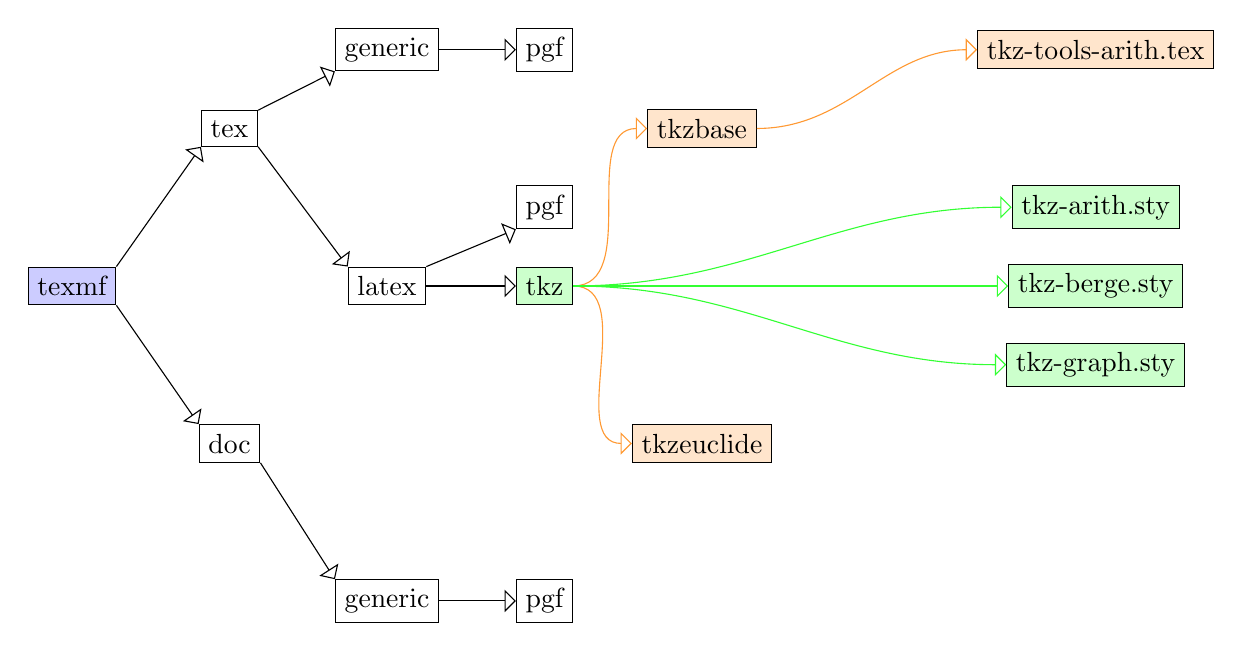
\begin{tikzpicture} [remember picture,rotate=90] 
% nodes
\node (texmf)   at (4,2)   [draw,fill=blue!20 ] {texmf};

\node (tex)     at (6,0)   [draw ] {tex}; 
\node (doc)     at (2,0)   [draw ] {doc};

\node (texgen)  at (7,-2)  [draw ] {generic};
\node (docgen)  at (0,-2)  [draw ] {generic};

\node (latex)   at (4,-2)  [draw ] {latex}; 

\node (genpgf)  at (7,-4)  [draw] {pgf};
\node (latpgf)  at (5,-4)  [draw] {pgf};
\node (tkz)     at (4,-4)  [draw,fill=green!20 ] {tkz};

\node (docpgf)  at (0,-4)  [draw] {pgf};

\node (tkb)     at (6,-6)  [draw,fill=orange!20]  {tkzbase};
\node (tke)     at (2,-6)  [draw,fill=orange!20]  {tkzeuclide};

\node (tari)    at (7,-11)  [draw,fill=orange!20] {tkz-tools-arith.tex};   
\node (tary)    at (5,-11)  [draw,fill=green!20]  {tkz-arith.sty};
\node (tgra)    at (4,-11)  [draw,fill=green!20]  {tkz-berge.sty}; 
\node (tber)    at (3,-11)  [draw,fill=green!20]  {tkz-graph.sty};

% edges
\draw[-open triangle 90](texmf.north east) -- (tex.south west)    ;
\draw[-open triangle 90](texmf.south east) -- (doc.north west)    ;
                                                                  
\draw[-open triangle 90](tex.north east)   -- (texgen.south west) ;
\draw[-open triangle 90](tex.south east)   -- (latex.north west)  ; 
\draw[-open triangle 90](texgen.east)      -- (genpgf.west)       ;  
                                                                  
\draw[-open triangle 90](doc.south east)   -- (docgen.north west) ; 
\draw[-open triangle 90](docgen.east)      -- (docpgf.west)       ; 

\draw[-open triangle 90](latex.north east) -- (latpgf.south west) ; 
\draw[-open triangle 90](latex.east)       -- (tkz.west)          ;    
 
\draw[-open triangle 90,orange!80](tkz.east) to [out=-90,in=90](tkb.west)  ; 
\draw[-open triangle 90,orange!80](tkz.east) to [out=-90,in=90](tke.west)  ; 
\draw[-open triangle 90,orange!80](tkb.east) to [out=-90,in=90](tari.west) ; 
\draw[-open triangle 90,green!80](tkz.east) to [out=-90,in=90](tary.west) ; 
\draw[-open triangle 90,green!80](tkz.east) to [out=-90,in=90](tgra.west) ; 
\draw[-open triangle 90,green!80](tkz.east) to [out=-90,in=90](tber.west) ;  

\end{tikzpicture}

\begin{tikzpicture}[remember picture,overlay]
        \path[->,thin,green!80,>=latex] (n1) edge [bend left] (tkz);
        \path[->,thin,green!80,>=latex] (n2) edge [bend left] (tgra);
\end{tikzpicture}     

\vfill
\newpage

\subsection{How to work with the tkz-\LaTeX-package under Windows?}
\NameDist{MikTeX}\NameSys{Windows XP}
Download and install the following files (if not yet done):
\begin{enumerate}

  \item the \LaTeX-system MiKTeX from

      \url{http://www.miktex.org/}.

      What file you need (e.g.
      \texttt{basic-miktex-2.7.2904.exe}) and how to install
      this program is explained there in the "Download"
      section of the respective version (current version is
      2.7). In general and as usual in windows, you run the
      setup process by starting the setup file :\newline (e.g.\texttt{basic-miktex-2.7.2904.exe}).

  \item Till Tantau's \LaTeX-package \texttt{pgf-tikZ} from

      \url{http://sourceforge.net/projects/pgf/}

      "For MiKTeX, use the update wizard [of MiKTeX] to
      install the (latest versions of the) packages called
      \texttt{pgf}, \texttt{xcolor}, and \texttt{xkeyval}."
      (cited from the pgf manual, contained in the files
      downloaded).
       \item the sty-files and the doc-files of Alain's tkz-package
            from the CTAN servers or

            \url{http://www.altermundus.fr/pages/download.html}.
                
      or
      
      \url{http://altermundus.com/pages/downloads/index.html}.
      
            To add the files to MiKTeX:

            \begin{itemize}
              \item add a directory \texttt{prof} in the
                  directory \colorbox{blue!30}{\texttt{[MiKTeX-dir]/tex/latex}},
                  e.g. in windows explorer,
              \item copy the sty-files in this directory
                  \texttt{tkz},
              \item update the MiKTeX system, ether by running
                  in a DOS shell the command\newline "\colorbox{red!30}{|mktexlsr -u|}" \newline or by clicking\newline
                  "\colorbox{red!30}{|Start/Programs/Miktex/Settings/General|}", then
                  push the button \colorbox{red!30}{|Refresh FNDB|}.
            \end{itemize}
      \end{enumerate}

\subsection{The next version} 

Actually, the package uses \tkzname{xkeyval}, in the next version I will use \tkzname{pgfkeys}. It's possible that the syntax should be modified. My first idea is to keep \tkzname{tkz-graph} and to create a new name for the next version like  \tkzname{tkz-graph-x}.

Some of the main macros used in the file \tkzname{tkz-tool-arith.tex} are now in the CVS version of PGF. With the next version of PGF, it would be possible to remove the   file \tkzname{tkz-tool-arith.tex}.
\endinput

%!TEX root = /Users/ego/Boulot/TKZ/tkz-berge/doc-us/TKZdoc-berge-main.tex 
%<–––––––––––––––––––––––––––––––––––––––––––––––––––––––––––––––––––––––––>
\section{Macros and Vertices}
%<–––––––––––––––––––––––––––––––––––––––––––––––––––––––––––––––––––––––––>
\subsection{\tkzcname{grEmptyCycle}}

\begin{NewMacroBox}{grEmptyCycle}{\oarg{local options}\var{order}}
\begin{tabular}{llc}
Arguments   &   & Definition              \\
\midrule
\TAline{order} {}{order of the graph}   
\bottomrule
\end{tabular}

\medskip
\begin{tabular}{llc}

Options   & default  & definition                                           \\
\midrule
\TOline{RA}     {4}      { radius  circle}               
\TOline{prefix} {a}      {prefix for vertices }         
\TOline{Math}   {false}  {math mode }                    
\bottomrule
\end{tabular}

\medskip
\emph{The number of nodes in a graph is called its order. The argument "order" is an integer superior to $1$. |RA| defines the radius of the circle.}
\end{NewMacroBox}


\bigskip
\subsubsection{Empty Cycle}
\begin{center}
\begin{tkzexample}[very small]
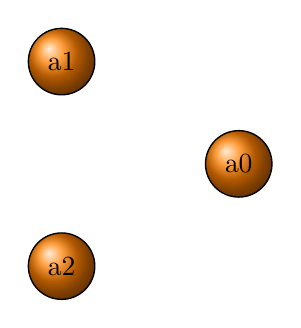
\begin{tikzpicture}
  \GraphInit[vstyle=Shade]
  \grEmptyCycle[RA=1.5]{3}
\end{tikzpicture}
\end{tkzexample}
\end{center}

\subsubsection{Empty Cycle  and \tkzcname{SetVertexNoLabel}}
\begin{center}
\begin{tkzexample}[very small]
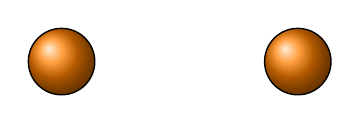
\begin{tikzpicture}
  \SetVertexNoLabel
  \GraphInit[vstyle=Shade]
  \grEmptyCycle[RA=1.5]{2}
\end{tikzpicture}
\end{tkzexample}
\end{center}

\subsubsection{Empty Cycle and \tkzname{Math}}
\begin{center}
\begin{tkzexample}[very small]
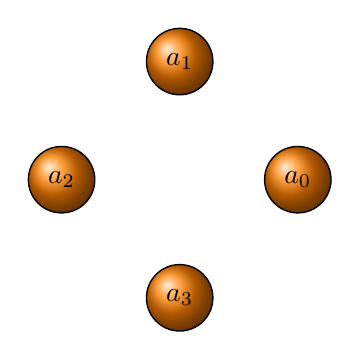
\begin{tikzpicture}
  \GraphInit[vstyle=Shade]
  \grEmptyCycle[Math,RA=1.5]{4}
\end{tikzpicture}
\end{tkzexample}
\end{center}


\subsubsection{Empty Cycle, \tkzcname{SetVertexMath} and \tkzname{prefix}}
\begin{center}
\begin{tkzexample}[very small]
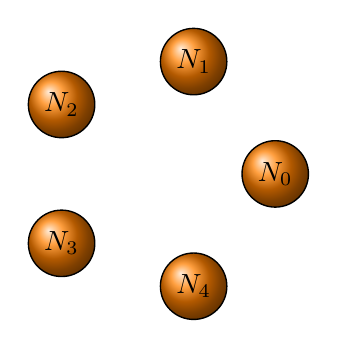
\begin{tikzpicture}
  \SetVertexMath
  \GraphInit[vstyle=Shade]
  \grEmptyCycle[prefix=N,RA=1.5]{5}
\end{tikzpicture}
\end{tkzexample}
\end{center}

\subsubsection{Empty Cycle and Classic style}
\begin{center}
\begin{tkzexample}[very small]
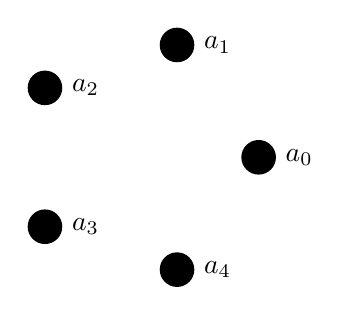
\begin{tikzpicture}
  \SetVertexMath
  \GraphInit[vstyle=Classic]
  \grEmptyCycle[RA=1.5]{5}
\end{tikzpicture}
\end{tkzexample}
\end{center}

\subsubsection{Empty Cycle and Simple style}
\begin{center}
\begin{tkzexample}[very small]
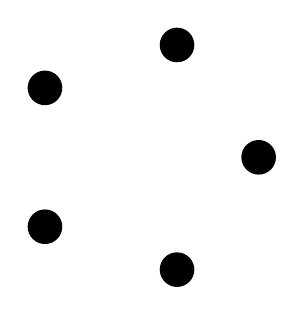
\begin{tikzpicture}
  \GraphInit[vstyle=Simple]
  \grEmptyCycle[RA=1.5]{5}
\end{tikzpicture}
\end{tkzexample}
\end{center}

\newpage
\subsection{\tkzcname{grEmptyPath}}
\begin{NewMacroBox}{grEmptyPath}{\oarg{local options}\var{order}}
\begin{tabular}{llc}
\hline
Arguments   &   & Definition              \\
\midrule
\TAline{order} {}{order of the graph}   
\bottomrule
\end{tabular}

\medskip
\begin{tabular}{>{\color{green!50!black}}lllc}
 \toprule 
options   & default  & definition                                           \\
\midrule
\TOline{RA}     {4 cm}{ distance between two vertices}               
\TOline{RS}     {? cm}{ distance between the first line  and the new one}    \\
\TOline{prefix} {a}      {prefix for vertices }          
\TOline{Math}   {false}  {math mode }                   
\bottomrule
\end{tabular}

\medskip
\emph{|Order| is the number of nodes. |RA| defines the radius of the circle.  |RS| defines the distance between the graph and the baseline.}

\end{NewMacroBox}

\bigskip
\tikzset{VertexStyle/.style = {shape        = circle,%
                               shading      = ball,%
                               ball color   = green!30,
                               minimum size = 24pt,
                               draw}}
\tikzset{EdgeStyle=      {color=red!30,
                           double= green!50!black,
                           double distance = 2pt}} 
\SetVertexLabel
\SetVertexMath
\subsubsection{Empty Path,   \tkzname{RA}  and \tkzname{Math}}
\begin{center}
\begin{tkzexample}[very small]
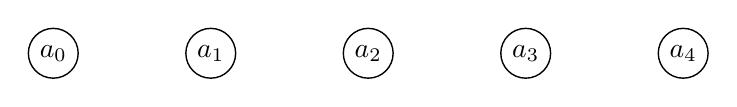
\begin{tikzpicture}
   \grEmptyPath[Math,RA=2]{5}
\end{tikzpicture}
\end{tkzexample}
\end{center}

\subsubsection{Empty Path,  \tkzname{RA}  and \tkzname{prefix}}
\begin{center}
\begin{tkzexample}[very small]
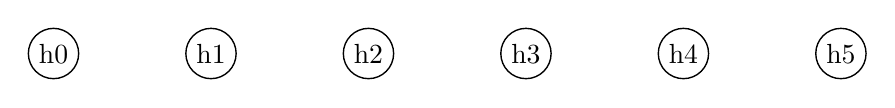
\begin{tikzpicture}
   \grEmptyPath[prefix=h,RA=2]{6}
\end{tikzpicture}
\end{tkzexample}
\end{center}

\subsubsection{Empty Path, vertical path with \tkzname{form=2}}
\begin{center}
\begin{tkzexample}[very small]
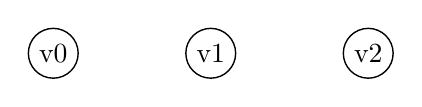
\begin{tikzpicture}
 \grEmptyPath[form=2,prefix=v,RA=2]{3}
\end{tikzpicture}
\end{tkzexample}
\end{center}


\subsubsection{Two Empty Paths}
\begin{center}  
\begin{tkzexample}[very small]
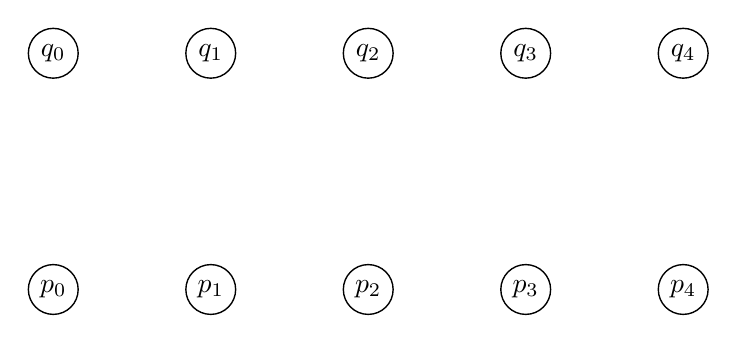
\begin{tikzpicture}
    \grEmptyPath[Math,prefix=p,RA=2,RS=0]{5}
    \grEmptyPath[Math,prefix=q,RA=2,RS=3]{5}
\end{tikzpicture}
\end{tkzexample}
\end{center}

\begin{center}  
\begin{tkzexample}[vbox]
\begin{tikzpicture}
    \grEmptyPath[Math,prefix=p,RA=2,RS=0,form=2]{5}
    \grEmptyPath[Math,prefix=q,RA=2,RS=4,form=2]{5}
\end{tikzpicture}
\end{tkzexample}
 \end{center}

\subsubsection{How to move a graph ?}
  \GraphInit[vstyle=Shade]
  \SetGraphShadeColor{blue!60!black!30}{blue}{white}
\begin{center}
\begin{tkzexample}[very small]
\begin{tikzpicture}
     \grPath[Math,prefix=u,RA=2,RS=0]{4}
     \grPath[Math,prefix=v,RA=2,RS=3]{4}
     \begin{scope}[xshift=1 cm]
      \grPath[Math,prefix=t,RA=2,RS=5]{4}
     \end{scope}
     \begin{scope}[shift={(4 cm,8cm)}]
      \grPath[Math,prefix=x,RA=2,RS=0]{4}
     \end{scope}
\end{tikzpicture}
\end{tkzexample}
\end{center}

\newpage 
\subsection{Empty Star}
\begin{NewMacroBox}{grEmptyStar}{\oarg{local options}\var{order}}
\begin{tabular}{llc}
 \toprule 
Arguments   &   & Definition              \\
\midrule
\TAline{order} {}{order of the graph}  
\bottomrule
\end{tabular}

\medskip
\begin{tabular}{>{\color{green!50!black}}lllc}
 \toprule 
options   & default  & definition                                           \\
\midrule
\TOline{RA}     {4 cm}{ radius circle}               
\TOline{prefix} {a}      {prefix for vertices }     
\TOline{Math}   {false}  {math mode }                
\bottomrule
\end{tabular}

\medskip
\emph{|RA| defines the radius of the circle. |order| is an integer and it's the order of the graph.}
\end{NewMacroBox}

\bigskip
\subsubsection{Empty Star}
\begin{center}
\begin{tkzexample}[very small]
\begin{tikzpicture}
  \SetVertexMath
  \grEmptyStar[prefix=s,RA=3]{6}
\end{tikzpicture}
\end{tkzexample}
\end{center}

\newpage 
\subsection{Empty Grid}
\begin{NewMacroBox}{grEmptyGrid}{\oarg{local options}\var{c}\var{r}}
\begin{tabular}{llc}
 \toprule 
Arguments   &   & Definition              \\
\midrule
\TAline{r} {}{number of rows}  
\TAline{c} {} {number of columns}  
\bottomrule
\end{tabular}

\medskip
\begin{tabular}{llc}
 \toprule 
options   & default  & definition                                           \\
\midrule
\TOline{RA}     {4 cm}{ distance between two columns }          
\TOline{RB} {3 cm}      {distance between two rows  }         
\TOline{prefix} {3 cm}      {distance between two rows  }     
\TOline{Math}   {false}  {math mode }                  
\bottomrule
\end{tabular}

\medskip
\emph{|c| and |r| are integers.}

\end{NewMacroBox}

 \bigskip
\subsubsection{Prefix}
\begin{center}
\begin{tkzexample}[very small]
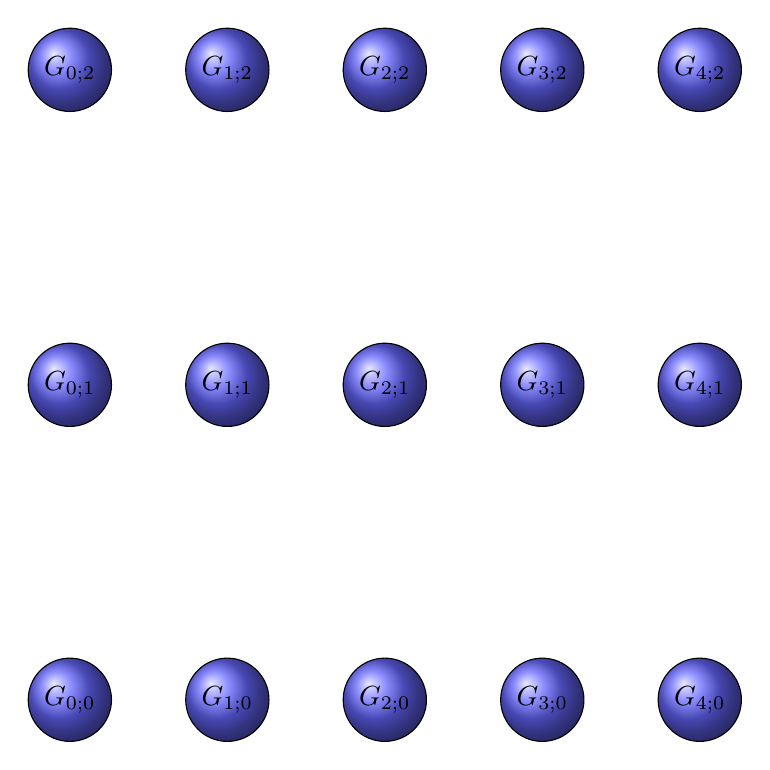
\begin{tikzpicture}
   \tikzset{VertexStyle/.style ={shape        = circle,
                                 shading      = ball,
                                 ball color   = Blue!60,%
                                 minimum size = 24pt,%
                                 draw}}
  \SetVertexMath
  \grEmptyGrid[prefix=G,RA=2,RB=4]{5}{3}
\end{tikzpicture}\end{tkzexample}
\end{center}

\newpage 
\subsection{Empty Ladder}
\begin{NewMacroBox}{grEmptyLadder}{\oarg{local options}\var{c}}
\begin{tabular}{llc}
 \toprule 
Arguments   &   & Definition              \\
\midrule
\TAline{c} {}{number of columns.}  
\bottomrule
\end{tabular}

\medskip
\begin{tabular}{llc}
options   & default  & definition                                           \\
 \midrule 
\TOline{RA}     {4 cm}{ distance between two columns  }           
\TOline{RB}     {3 cm}{ distance between two rows  }               
\TOline{prefix} {a}      {prefix for vertices }         
\TOline{prefix} {b}      {prefix for vertices }         
\TOline{Math}   {false}  {math mode }                    
\bottomrule
\end{tabular}

\medskip
 \emph{ |c| is an integer. There are only two rows with different prefix.}
\end{NewMacroBox}
 
\bigskip
\subsubsection{Empty Ladder}
\begin{center}
\begin{tkzexample}[very small]
\begin{tikzpicture}
   \tikzset{VertexStyle/.style ={shape        = diamond, 
                                 shading      = ball,
                                 ball color   = yellow!60,%
                                 minimum size = 24pt,%
                                 draw}}
   \SetVertexMath
   \grEmptyLadder[RA=2,RB=4]{5}
\end{tikzpicture}
\end{tkzexample}
\end{center}

 
\endinput



%!TEX root = /Users/ego/Boulot/TKZ/tkz-berge/doc-us/TKZdoc-berge-main.tex 

%<–––––––––––––––––––––––––––––––––––––––––––––––––––––––––––––––––––––––––>
\section{Macros and Edges in a graph}
%<–––––––––––––––––––––––––––––––––––––––––––––––––––––––––––––––––––––––––>
\subsection{Edge in a graph from one vertex \tkzcname{EdgeInGraphFromOneToComp}}

\begin{NewMacroBox}{EdgeInGraphFromOneToComp}{\oarg{local options}\var{prefix}\var{order}\var{from}}
   
\begin{tabular}{llc}
\hline
Arguments   &   & Definition              \\
\midrule
\TAline{order} {}{order of the graph}  
\bottomrule
\end{tabular}

\medskip
\begin{tabular}{llc}
\midrule
options   & default  & definition                                           \\
\midrule
\TOline{RA}     {4}      { radius  circle}            
\TOline{prefix} {a}      {prefix for vertices }       
\TOline{Math}   {false}  {math mode }                
\bottomrule
\end{tabular}

\medskip
\emph{This macro works on an unique graph. |from| is integer. |EdgeInGraph| designs a macro that works only in a graph defined by a prefix. The result is some edges between the vertex |from| and the others vertices. }
\end{NewMacroBox}





\subsubsection{Empty Cycle}
\begin{center}
\begin{tkzexample}[very small]
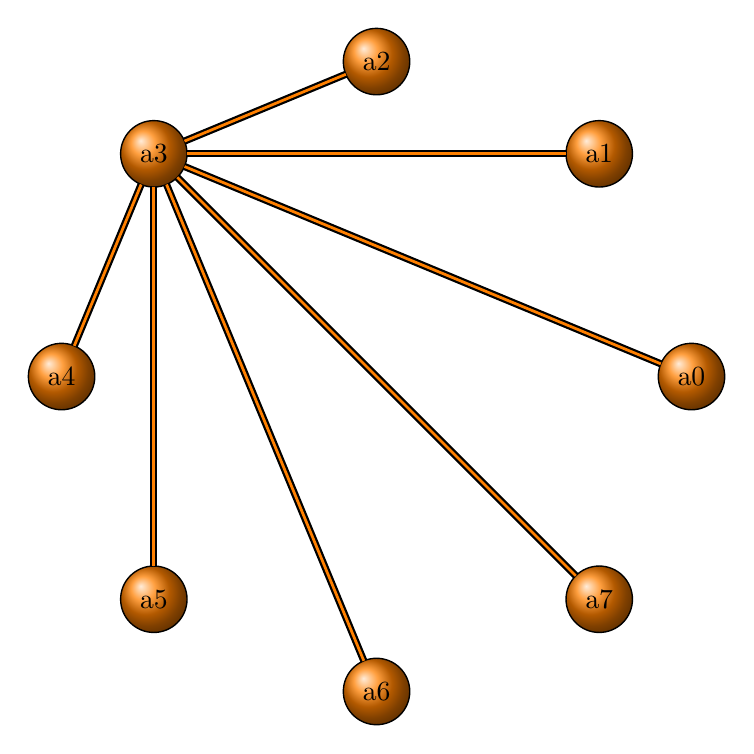
\begin{tikzpicture}
  \GraphInit[vstyle=Shade]
  \grEmptyCycle[RA=4,prefix=a]{8}% 
  \EdgeInGraphFromOneToComp{a}{8}{3} 
\end{tikzpicture}
\end{tkzexample}
\end{center}
 
\vfill
\newpage
\subsection{Edges in a graph - a loop \tkzcname{EdgeInGraphLoop}}%
\begin{NewMacroBox}{EdgeInGraphLoop}{\var{prefix}\var{order}}
\emph{This macro is useful with vertices on a circle . |order| in an integer.}
\end{NewMacroBox} 


\subsubsection{Empty Cycle}
\begin{center}
  \begin{tkzexample}[very small]
  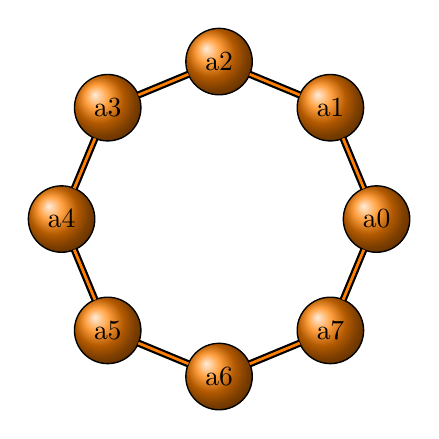
\begin{tikzpicture}
  \GraphInit[vstyle=Shade]
  \grEmptyCycle[RA=2,prefix=a]{8}% 
  \EdgeInGraphLoop{a}{8} 
  \end{tikzpicture}\end{tkzexample}
\end{center}

\subsubsection{Empty Cycle}
\begin{center}
\begin{tkzexample}[very small]
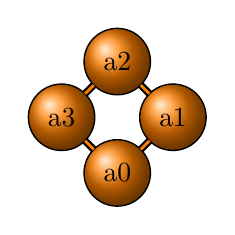
\begin{tikzpicture}[node distance=4cm]
 \GraphInit[vstyle=Shade]
 \Vertices{square}{a0,a1,a2,a3}
 \EdgeInGraphLoop{a}{4}
\end{tikzpicture}
\end{tkzexample}
\end{center}

\newpage
\subsection{Edges in a graph - a loop \tkzcname{EdgeInGraphLoop*}}
\begin{NewMacroBox}{EdgeInGraphLoop*}{\var{prefix}\var{order}}

\medskip
\emph{Not exactly a loop, there is no edge between the first and the last vertex.}
\end{NewMacroBox}

\subsubsection{Empty Cycle}
\begin{center}
\begin{tkzexample}[very small]
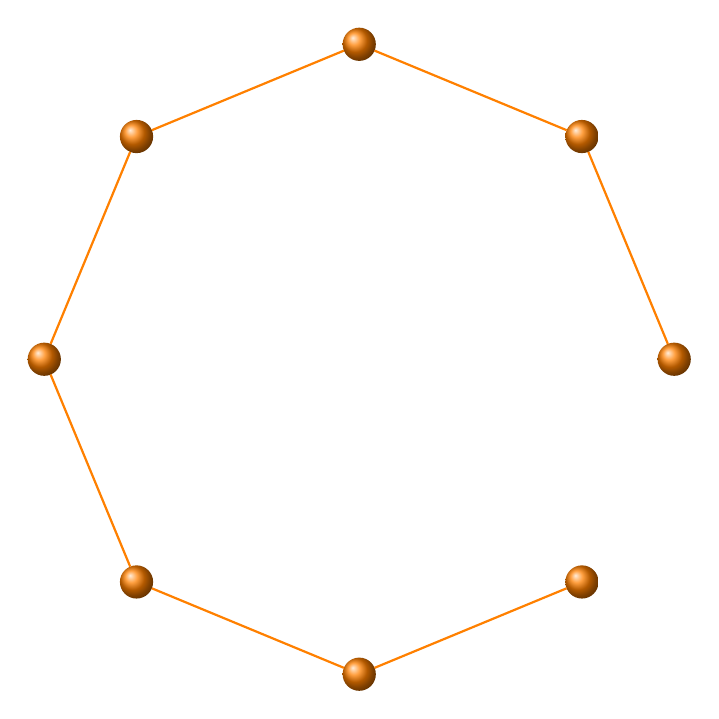
\begin{tikzpicture}
  \GraphInit[vstyle=Art]
  \grEmptyCycle[RA=4,prefix=a]{8}% 
  \EdgeInGraphLoop*{a}{8} 
\end{tikzpicture}
\end{tkzexample}
\end{center}

\subsubsection{Empty Path}
\begin{center}
\begin{tkzexample}[very small]
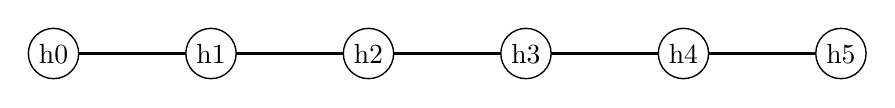
\begin{tikzpicture}
     \grEmptyPath[prefix=h,RA=2,RS=2]{6}
     \EdgeInGraphLoop*{h}{6}
\end{tikzpicture}
\end{tkzexample}
\end{center}

\vfill
\newpage  
\subsection{Sequence of edges in a graph  \tkzcname{EdgeInGraphSeq}}
\begin{NewMacroBox}{EdgeInGraphSeq}{\var{prefix}\var{start}\var{end}}

\medskip
\emph{This macro gives a sequence of edges between |start| and |end|.\\
|start| and |end| are  two integers. }
\end{NewMacroBox} 

\subsubsection{EdgeInGraphSeq}
\begin{center}
\begin{tkzexample}[very small]
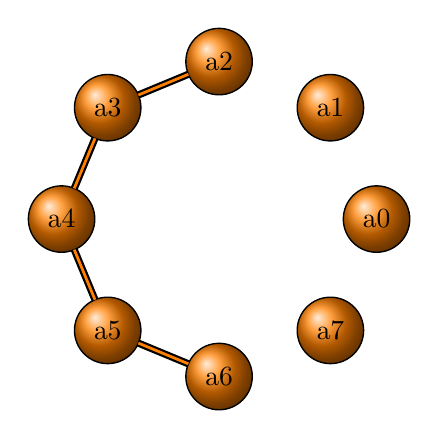
\begin{tikzpicture}
  \GraphInit[vstyle=Shade]
  \grEmptyCycle[RA=2,prefix=a]{8}% 
  \EdgeInGraphSeq{a}{2}{5}
\end{tikzpicture}
\end{tkzexample}
\end{center} 

\newpage
\subsection{Edges in a graph  \tkzcname{EdgeInGraphMod}}
\begin{NewMacroBox}{EdgeInGraphMod}{\var{prefix}\var{order}\var{add}}

\medskip
\emph{This macro works on an unique graph. Edges between $v_i$ and $v_j$ with $i$ in $0,...,(\text{\#2}-1)$  and $j=\text{Mod(i+\#3,\#2)}$.\\
\#2 = |order| and  \#3 = |add|.\\
|Mod| is like |mod| but the result is a positive integer. }
\end{NewMacroBox} 

\subsubsection{EdgeInGraphMod}
\begin{center}
\begin{tkzexample}[very small]
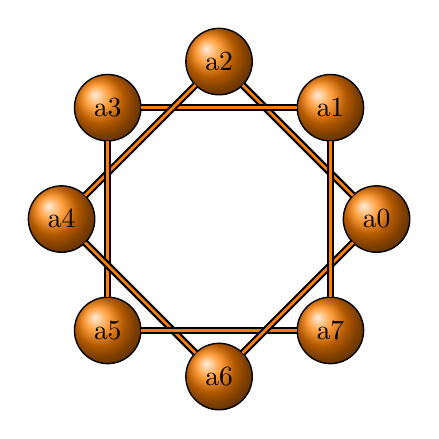
\begin{tikzpicture}
  \GraphInit[vstyle=Shade]
  \grEmptyCycle[RA=2,prefix=a]{8}% 
  \EdgeInGraphMod{a}{8}{2}
\end{tikzpicture}
\end{tkzexample}
\end{center}

\subsubsection{EdgeInGraphMod 2}
\begin{center}
\begin{tkzexample}[very small]
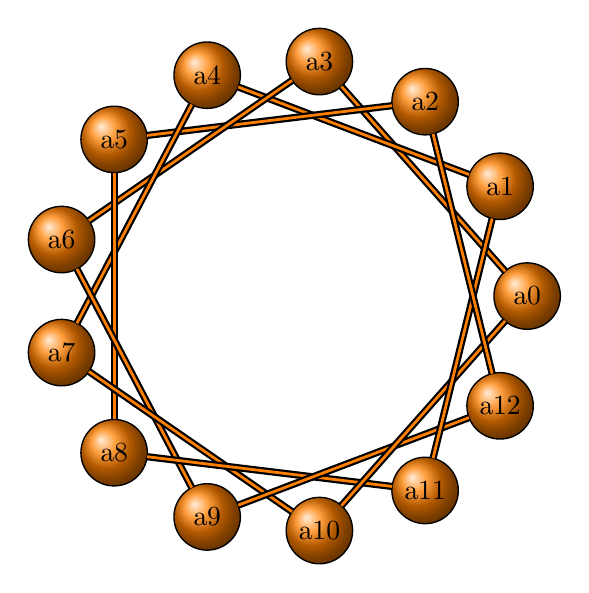
\begin{tikzpicture}
  \GraphInit[vstyle=Shade]
  \grEmptyCycle[RA=3,prefix=a]{13}% 
  \EdgeInGraphMod{a}{13}{3}
\end{tikzpicture}
\end{tkzexample}
\end{center}
 
\newpage
\subsection{Edges in a graph  \tkzcname{EdgeInGraphMod*}}
\begin{NewMacroBox}{EdgeInGraphMod*}{\var{prefix}\var{order}\var{add}\var{start}\var{step}}

\medskip
\emph{Edges between $v_i$ and $v_j$ with $i$ in $\#4,\#4+\#5,...,(\text{\#2}-1)$  and $j=\text{Mod(i+\#3,\#2)}$}\\
\#2 = |order|,  \#3 = |add|, \#4 = |start|, \#5 = |step|.\\
\end{NewMacroBox} 

\subsubsection{EdgeInGraphMod*}
\begin{center}
\begin{tkzexample}[very small]
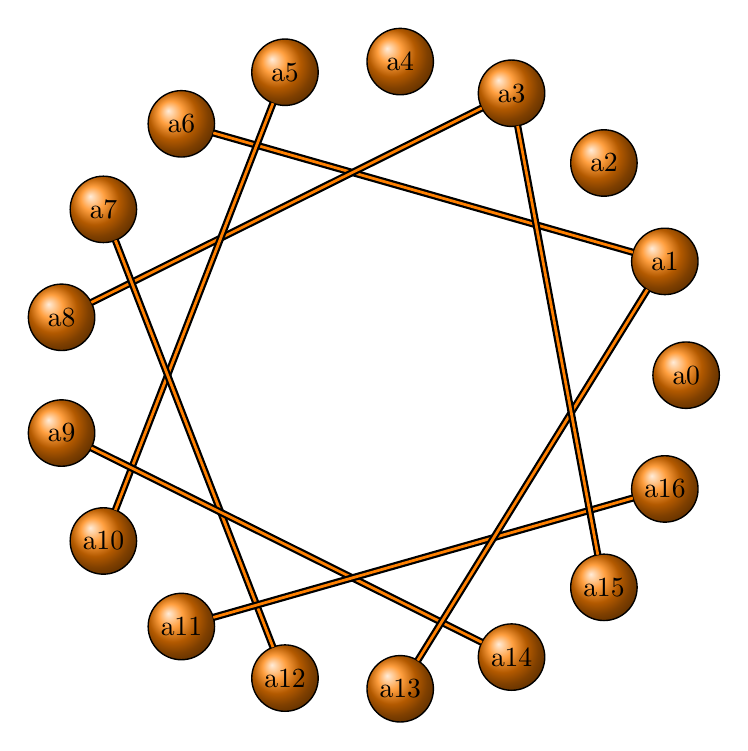
\begin{tikzpicture}
  \GraphInit[vstyle=Shade]
  \grEmptyCycle[prefix=a]{17}% 
  \EdgeInGraphMod*{a}{17}{5}{1}{2}
\end{tikzpicture}
\end{tkzexample}
\end{center}

\newpage
\subsection{Edges in a graph  \tkzcname{EdgeInGraphModLoop}}
\begin{NewMacroBox}{EdgeInGraphModLoop}{\var{prefix}\var{order}\var{add}\var{start}}

\medskip
\emph{ |order|, |add| and |start| are integers.\\
Edges between $v_i$ and $v_j$ with $i$ from $\#4$, $j=\text{Mod(i+\#3,\#2)}$ and then $i=j$ until $j=\#4$\\
\#2 = |order|,  \#3 = |add| and \#4 = |start|.}
\end{NewMacroBox}

\subsubsection{EdgeInGraphModLoop}
\begin{center}
\begin{tkzexample}[very small]
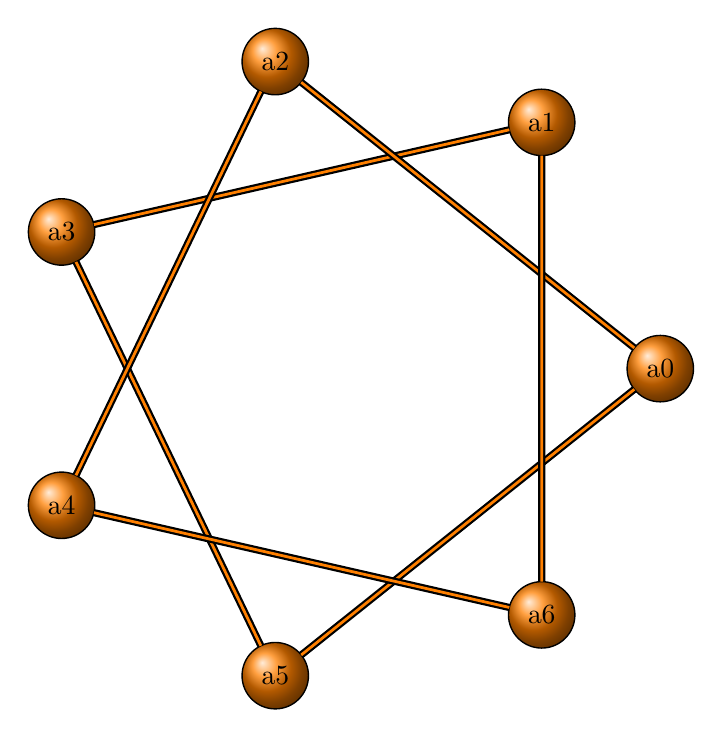
\begin{tikzpicture}
  \GraphInit[vstyle=Shade]
  \grEmptyCycle[RA=4]{7} 
  \EdgeInGraphModLoop{a}{7}{2}{1} 
\end{tikzpicture}
\end{tkzexample}
\end{center}

\subsubsection{EdgeInGraphModLoop}
\begin{center}
\begin{tkzexample}[very small]
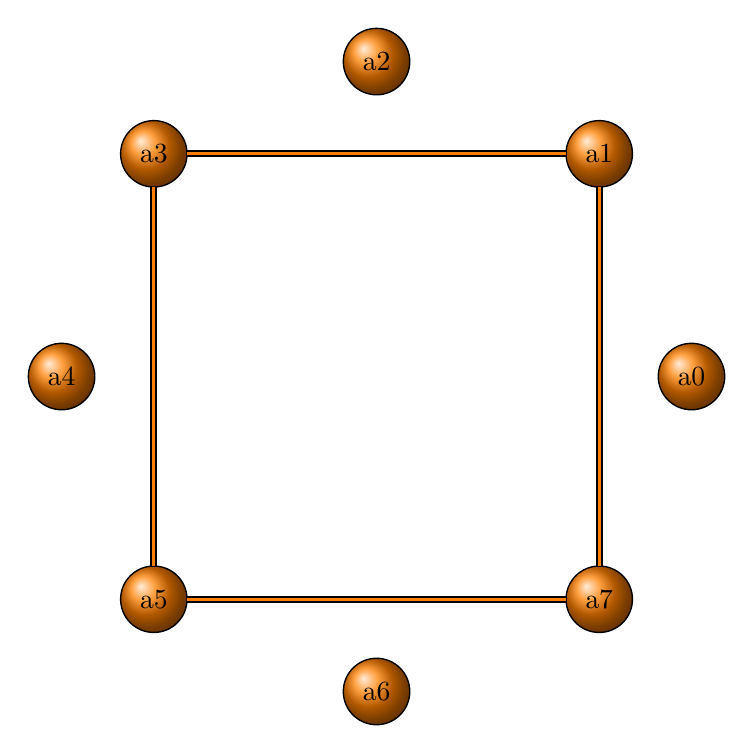
\begin{tikzpicture}
  \GraphInit[vstyle=Shade]
  \grEmptyCycle[RA=4]{8} 
  \EdgeInGraphModLoop{a}{8}{2}{1} 
\end{tikzpicture}
\end{tkzexample}
\end{center}


\newpage
\subsection{Edges between two graphs with the same order \tkzcname{EdgeIdentity}}

\begin{NewMacroBox}{EdgeIdentity}{\var{prefix1}\var{prefix2}\var{order}}

\medskip
\emph{|order| is an integer. This macro gives edges between two graphs.\\
Edges between $v_i$ and $v_j$ with $i=j$ in $0,...,(\text{\#3}-1)$.\\
\#3 = |order|.\\}
\end{NewMacroBox}  

\subsubsection{EdgeIdentity}
\begin{center}
\begin{tkzexample}[very small]
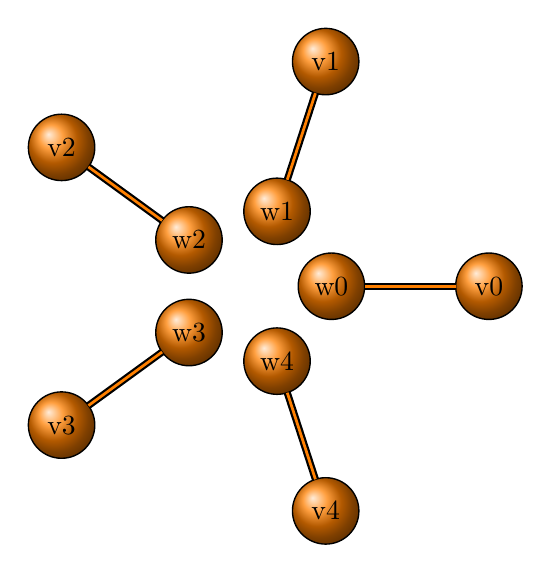
\begin{tikzpicture}
  \GraphInit[vstyle=Shade]
    \grEmptyCycle[prefix=v,RA=3]{5}
    \grEmptyCycle[prefix=w,RA=1]{5}
    \EdgeIdentity{v}{w}{5}
\end{tikzpicture}
\end{tkzexample}
\end{center}
 
\vfill
\newpage  
\subsection{Edges between two graphs with the same order \tkzcname{EdgeIdentity*}}

\begin{NewMacroBox}{EdgeIdentity*}{\var{prefix1}\var{prefix2}\var{list}}

\medskip
\emph{|list| is a list of  integers. This macro gives edges between two graphs.\\
Edges between $v_i$ and $v_j$ with $i=j$ in |list|.\\}

\end{NewMacroBox}

\subsubsection{EdgeIdentity*}
\begin{center}
\begin{tkzexample}[very small]
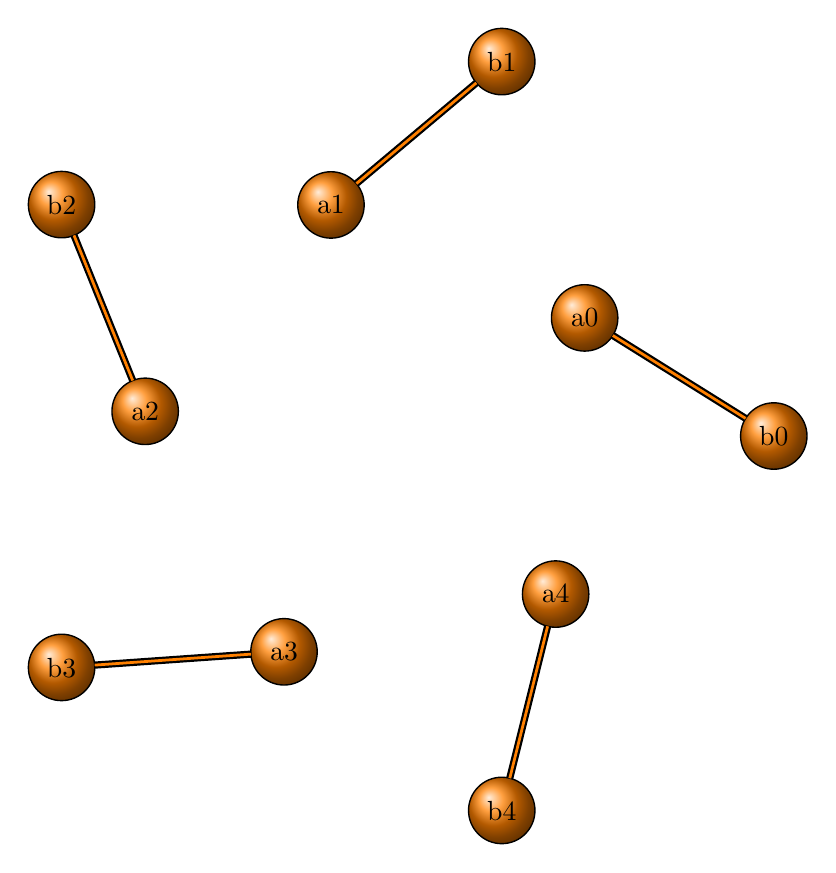
\begin{tikzpicture}
  \GraphInit[vstyle=Shade]
  \begin{scope}[rotate=30]
  \grEmptyCycle[RA=3,prefix=a]{5}%
  \end{scope}
  \grEmptyCycle[RA=5,prefix=b]{5}%
   \EdgeIdentity*{a}{b}{0,...,4}    
\end{tikzpicture}
\end{tkzexample}
\end{center}

\subsubsection{EdgeIdentity*}
\begin{center}
\begin{tkzexample}[very small]
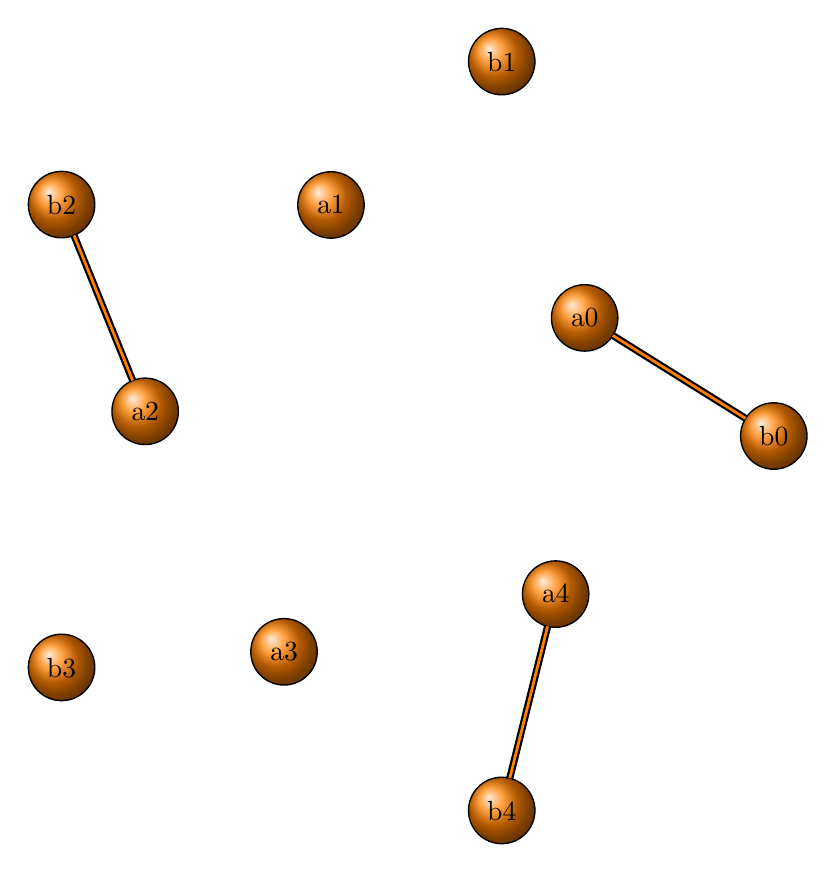
\begin{tikzpicture}
 \GraphInit[vstyle=Shade]
  \begin{scope}[rotate=30]
  \grEmptyCycle[RA=3,prefix=a]{5}%
  \end{scope}
  \grEmptyCycle[RA=5,prefix=b]{5}%
   \EdgeIdentity*{a}{b}{0,2,4}    
\end{tikzpicture}
\end{tkzexample}
\end{center}

\newpage
\subsection{Edges between two graphs \tkzcname{EdgeFromOneToAll}}
\begin{NewMacroBox}{EdgeFromOneToAll}{\var{prefix1}\var{prefix2}\var{from}\var{order}}

\medskip
\emph{The graphs must to have the same order. |from| and |order| are integers.}
\end{NewMacroBox}

\subsubsection{EdgeFromOneToAll}
\begin{center}
\begin{tkzexample}[very small]
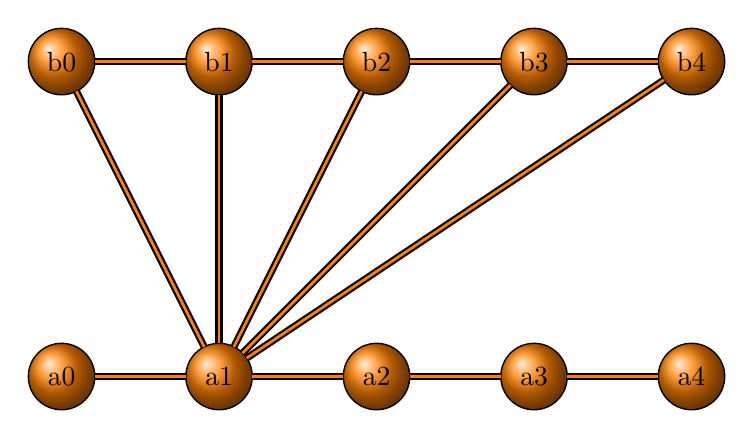
\begin{tikzpicture}
  \GraphInit[vstyle=Shade]
  \grPath[form=1,RA=2,RS=0]{5}
  \grPath[form=1,prefix=b,RA=2,RS=4]{5}
  \EdgeFromOneToAll{a}{b}{1}{5} 
\end{tikzpicture}\end{tkzexample}
\end{center}

\newpage
\subsection{Edges between two graphs \tkzcname{EdgeFromOneToSeq}}
\begin{NewMacroBox}{EdgeFromOneToSeq}{\var{prefix1}\var{prefix2}\var{from}\var{start}\var{end}}

\medskip
\emph{|from|, |start| and |end| are integers. This macro  builds edges between the vertex with an indice |from| through the vertices with an indice in the sequence |start|,...,|end|.}
\end{NewMacroBox} 

\subsubsection{EdgeFromOneToSeq}
\begin{center}
\begin{tkzexample}[very small]
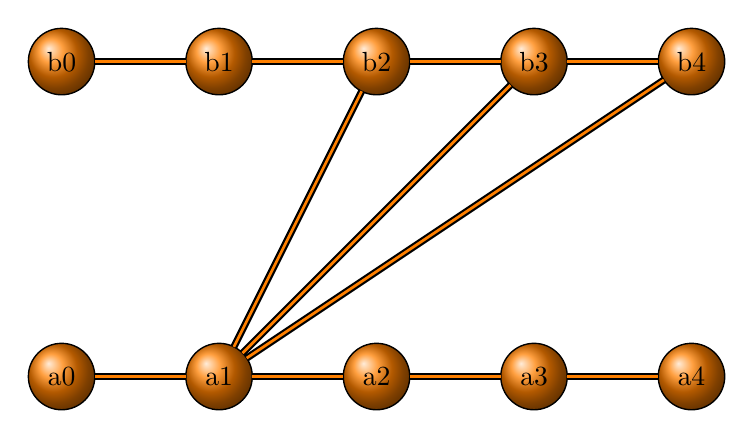
\begin{tikzpicture}
  \GraphInit[vstyle=Shade]
  \grPath[form=1,RA=2,RS=0]{5}
  \grPath[form=1,prefix=b,RA=2,RS=4]{5}
  \EdgeFromOneToSeq{a}{b}{1}{2}{4} 
\end{tikzpicture}
\end{tkzexample}
\end{center}

\newpage
\subsection{Edges between two graphs \tkzcname{EdgeFromOneToSel}}
\begin{NewMacroBox}{EdgeFromOneToSel}{\var{prefix1}\var{prefix2}\var{from}\var{list}}

\medskip
\emph{This macro  builds edges between the vertex with an indice |from| through the vertices with an indice in the list |list|.}
\end{NewMacroBox} 


\subsubsection{EdgeFromOneToSel}
\begin{center}
\begin{tkzexample}[very small]
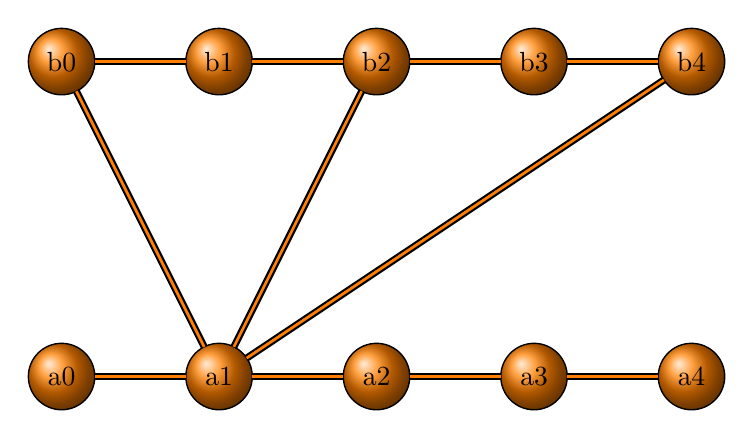
\begin{tikzpicture}
  \GraphInit[vstyle=Shade]
  \grPath[form=1,RA=2]{5}
  \grPath[form=1,prefix=b,RA=2,RS=4]{5} 
  \EdgeFromOneToSel{a}{b}{1}{0,2,4} 
\end{tikzpicture}
\end{tkzexample}
\end{center}

\newpage  
\subsection{Edges between two graphs \tkzcname{EdgeFromOneToComp}}
\begin{NewMacroBox}{EdgeFromOneToComp}{\var{prefix1}\var{prefix2}\var{from}\var{order2}}

\medskip
\emph{This macro  builds edges between the vertex with an indice |from| through all the vertices of the second graph, except the vertex with an indice |from|.}
\end{NewMacroBox}  

\subsubsection{EdgeFromOneToComp}
\begin{center}
\begin{tkzexample}[vbox]
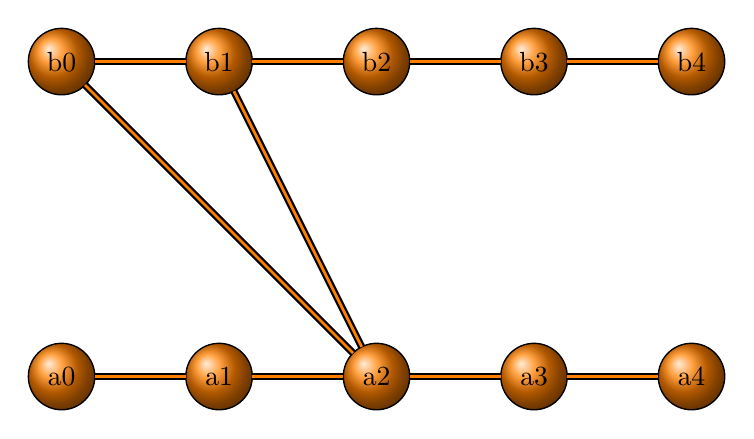
\begin{tikzpicture}
  \GraphInit[vstyle=Shade]
  \grPath[form=1,RA=2,RS=0]{5}
  \grPath[form=1,prefix=b,RA=2,RS=4]{5}
  \EdgeFromOneToComp{a}{b}{2}{3} 
\end{tikzpicture}
\end{tkzexample}
\end{center}

\newpage  
\subsection{Edges between two graphs \tkzcname{EdgeMod}}%
\begin{NewMacroBox}{EdgeMod}{\var{prefix1}\var{prefix2}\var{order}\var{step}}

\medskip
\emph{This macro works on two graphs with the same order. We get edges between $v_i$ and $v_j$ with $i$ in $0,...,(\text{\#2}-1)$  and $j=\text{Mod(i+\#4,\#3)}$.\\
\#3 = |order| and  \#4 = |step|.}
\end{NewMacroBox}  

\subsubsection{EdgeMod}
\begin{center}
\begin{tkzexample}[vbox]
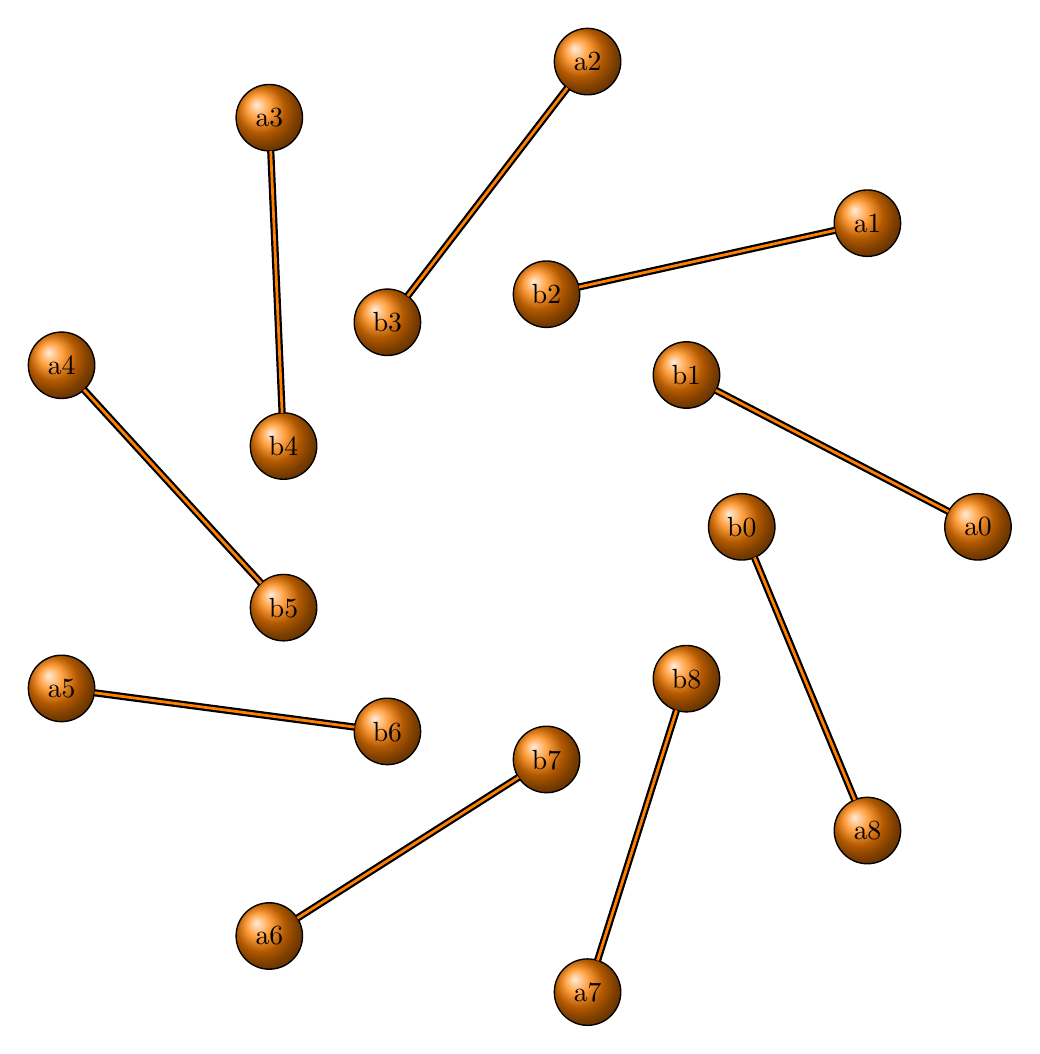
\begin{tikzpicture}
 \GraphInit[vstyle=Shade]
 \grEmptyCycle[prefix=a,RA=6]{9}
 \grEmptyCycle[prefix=b,RA=3]{9}
 \EdgeMod{a}{b}{9}{1}
\end{tikzpicture}
\end{tkzexample}
\end{center}

\newpage  
\subsection{Edges between two graphs \tkzcname{EdgeMod*}}%
\begin{NewMacroBox}{EdgeMod*}{\var{prefix1}\var{prefix2}\var{order}\var{step1}\var{step2}}

\medskip
\emph{This macro works on two graphs with the same order. We get edges between $v_i$ and $v_j$ with $i$ in $0,...,(\text{\#3}-1)$ with a step $\text{\#5}$ and $j=\text{Mod(i+\#4,\#3)}$.\\
\#3 = |order| ,  \#4 = |step1| and \#5 = |step2|.}
\end{NewMacroBox}  


\subsubsection{\tkzcname{EdgeMod*} }%with |step1|=1 and |step2|=2
\begin{center}
\begin{tkzexample}[vbox]
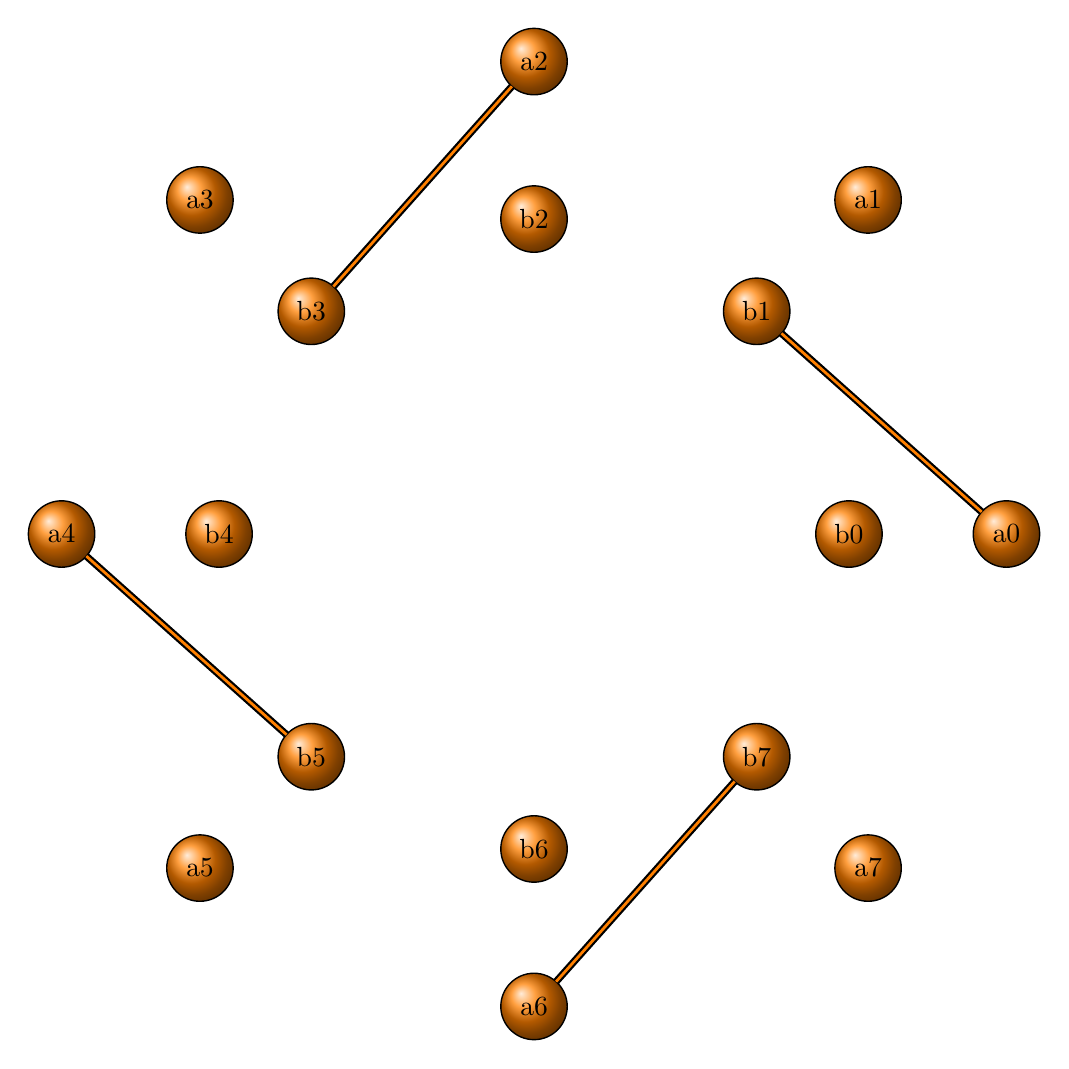
\begin{tikzpicture}
 \GraphInit[vstyle=Shade]
 \grEmptyCycle[prefix=a,RA=6]{8}
 \grEmptyCycle[prefix=b,RA=4]{8}
 \EdgeMod*{a}{b}{8}{1}{2}
\end{tikzpicture}
\end{tkzexample}
\end{center}


\subsubsection{EdgeMod* }%with |step1|=2 and |step2|=1
\begin{center}
\begin{tkzexample}[vbox] 
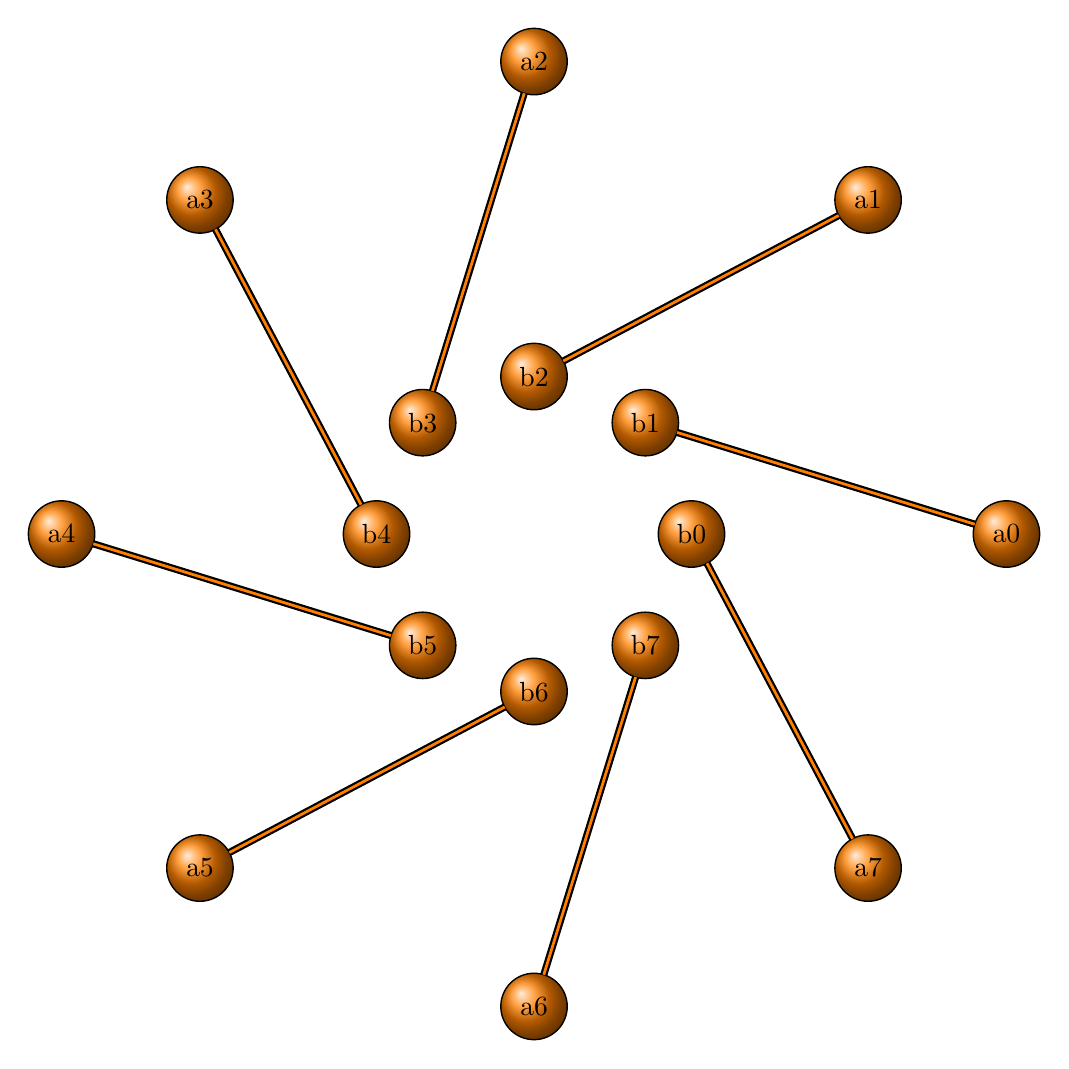
\begin{tikzpicture}
 \GraphInit[vstyle=Shade]
 \grEmptyCycle[prefix=a,RA=6]{8}
 \grEmptyCycle[prefix=b,RA=2]{8}
 \EdgeMod*{a}{b}{8}{1}{1}
\end{tikzpicture}
\end{tkzexample}
\end{center}

\newpage  
\subsection{Edges between two graphs \tkzcname{EdgeDoubleMod}}%
\begin{NewMacroBox}{EdgeDoubleMod}{\var{prefix1}\var{nb}\var{nb}\var{nb}\var{prefix2}\var{nb}\var{nb}\var{nb}\var{end}}

For the first node,  the numbers are :
\var{order1}\var{start1}\var{add1}

\medskip  
For the second node,  the numbers are :  
\var{order2}\var{start2}\var{add2}\var{end} 
  
\medskip
\emph{Edges between $v_i$ and $v_j$ with $i=\text{Mod(\#3+(\#4*k),\#2)}$ and j=$\text{Mod(\#7+(\#8*k),\#6)}$ $k$ is an integer from $0$ to |end|.\\
\#2 = |order1|,  \#3 = |start1| and \#4 = |add1|.\\
\#6 = |order2|,  \#7 = |start2| and \#8 = |add2|.}
\end{NewMacroBox} 


\subsubsection{EdgeDoubleMod}
\begin{center}
\begin{tkzexample}[vbox]
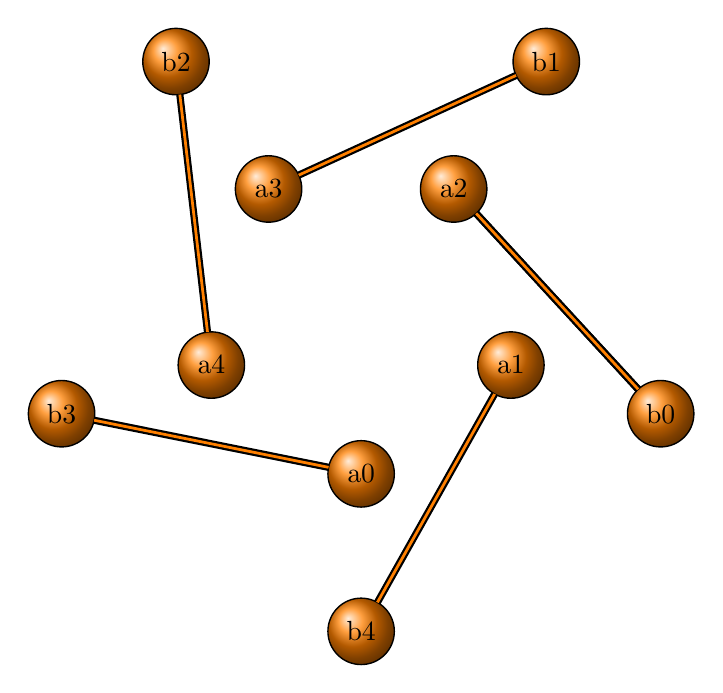
\begin{tikzpicture}
  \GraphInit[vstyle=Shade]
    \begin{scope}[rotate=-90]
      \grEmptyCycle[RA=2,prefix=a]{5}{2}
    \end{scope}
    \begin{scope}[rotate=-18]
      \grEmptyCycle[RA=4,prefix=b]{5}{2}
    \end{scope}
    \EdgeDoubleMod{b}{5}{0}{1}%
                 {a}{5}{2}{1}{5}
\end{tikzpicture}
\end{tkzexample}
\end{center}


\subsubsection{EdgeDoubleMod with two graphs and different orders}
\begin{center}
\begin{tkzexample}[vbox]
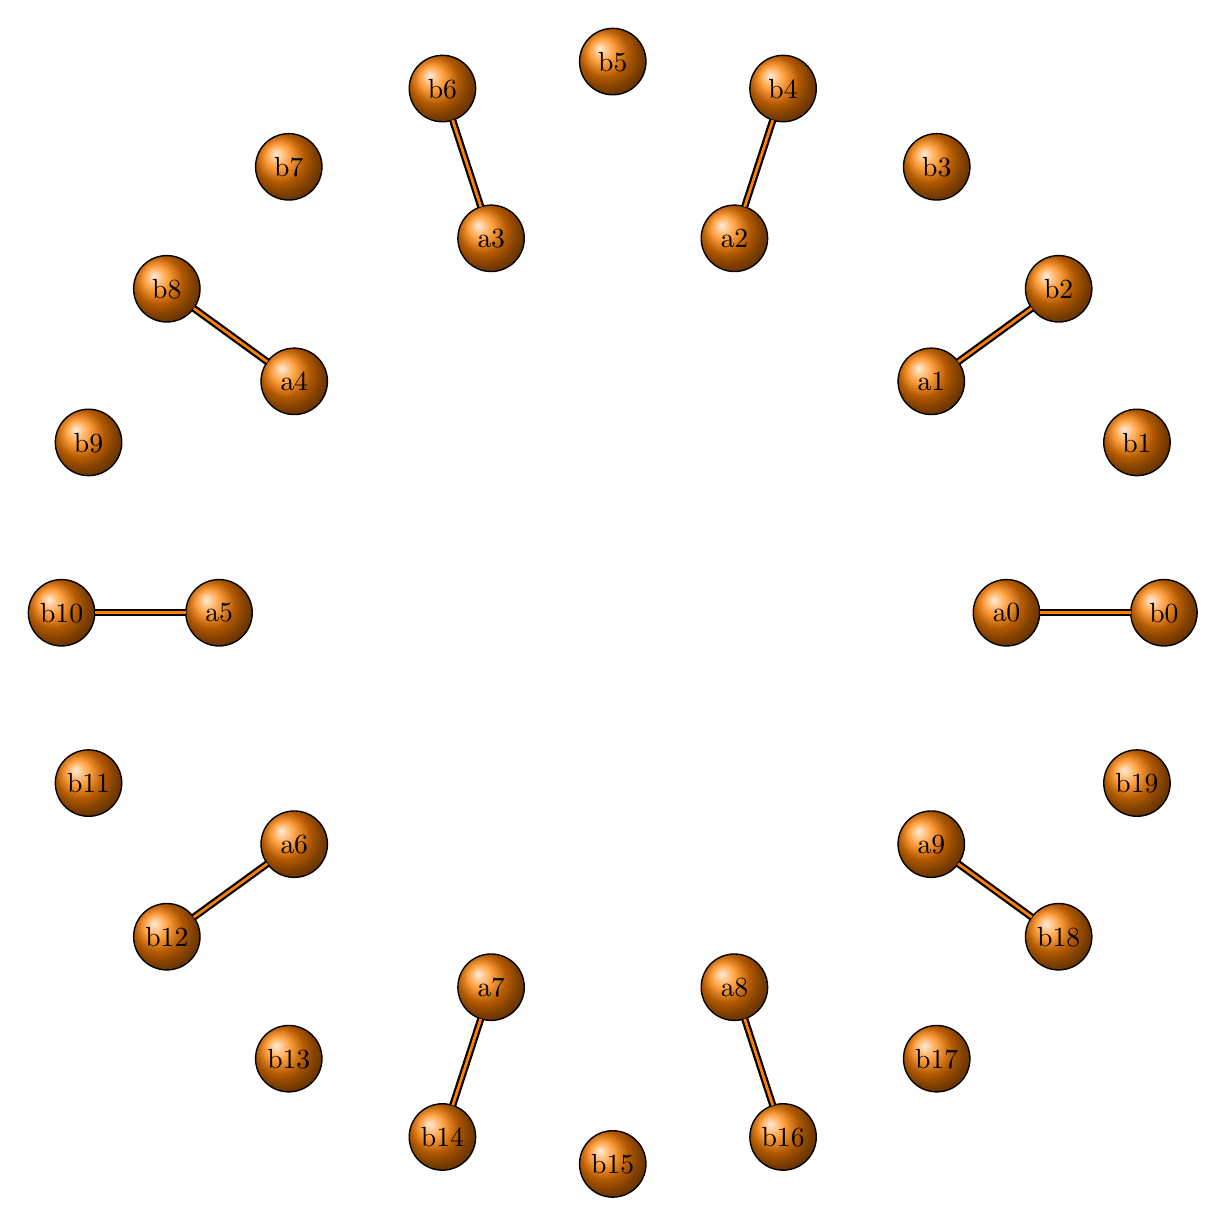
\begin{tikzpicture}
  \GraphInit[vstyle=Shade]
  \grEmptyCycle[prefix=a,RA=5]{10}
  \grEmptyCycle[prefix=b,RA=7]{20}
   \EdgeDoubleMod{a}{10}{0}{1}%
                 {b}{20}{0}{2}{10}
\end{tikzpicture}
\end{tkzexample}
\end{center}
\endinput
 
%!TEX root = /Users/ego/Boulot/TKZ/tkz-berge/doc-us/TKZdoc-berge-main.tex
%<–––––––––––––––––––––––––––––––––––––––––––––––––––––––––––––––––––––––––>
\section{Classic Graphs}
%<–––––––––––––––––––––––––––––––––––––––––––––––––––––––––––––––––––––––––>
%<–––––––––––––––––––––––     graphes classiques    –––––––––––––––––––––––––>
%<–––––––––––––––––––––––––––––––––––––––––––––––––––––––––––––––––––––––––––>
\subsubsection{Cycle graph}
\begin{NewMacroBox}{grCycle}{\oarg{local options}\var{order}}

\medskip
\emph{A cycle graph $C_n$ is a graph on $n$ nodes containing a single cycle through all nodes. Cycle graphs can be generated using \tkzcname{grCycle} in   the \tkzname{tkz-berge.sty} package. Special cases include  the triangle graph and  the square graph.}

\medskip
External links :

\medskip
\begin{itemize}

\item \href{http://mathworld.wolfram.com/CycleGraph.html}%
           {\textcolor{blue}{MathWorld - CycleGraph}} by %
      \href{http://en.wikipedia.org/wiki/Eric_W._Weisstein}%
           {\textcolor{blue}{E.Weisstein}}

\item  \href{http://en.wikipedia.org/wiki/Cycle_graph}%
            {\textcolor{blue}{Wikipedia}}

\end{itemize}
\end{NewMacroBox} 

\subsubsection{Special cases : the triangle graph and  the square graph}


\begin{center}
\begin{tkzexample}[small]
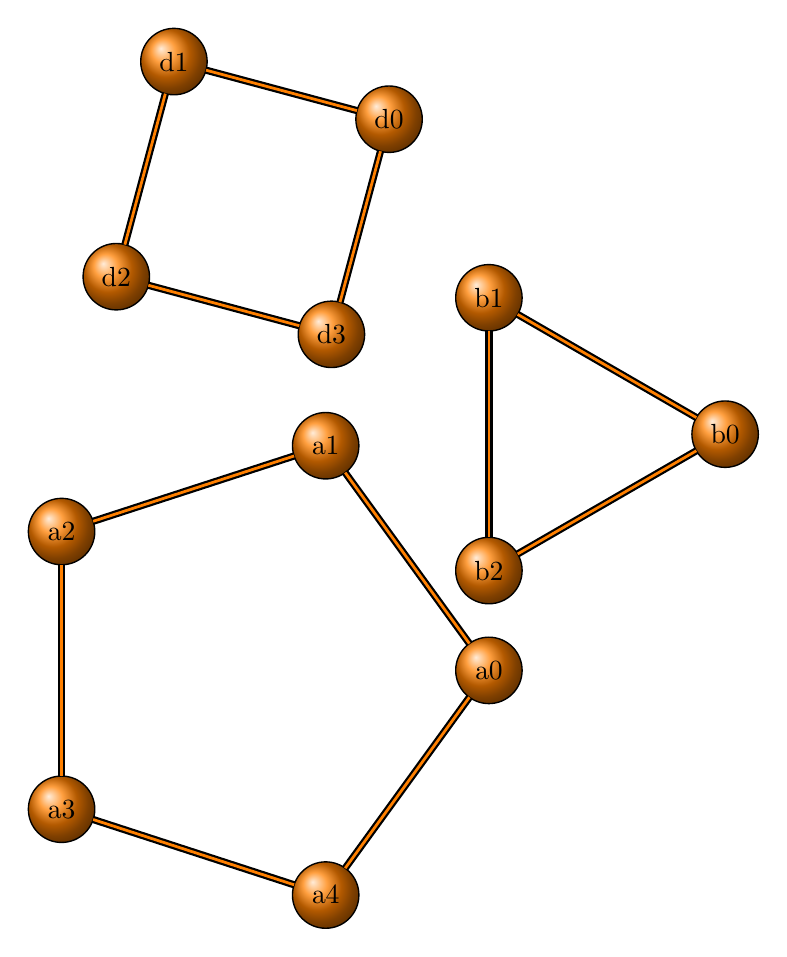
\begin{tikzpicture}
    \GraphInit[vstyle=Shade] 
    \grCycle[prefix=a,RA=3]{5}
    \grCycle[x=4,y=3,prefix=b,RA=2]{3}
    \grCycle[prefix=d,y=6,rotation=30,RA=2]{4}
\end{tikzpicture}
\end{tkzexample} 
\end{center}
 
\newpage
\subsubsection{Complete graph} 
\begin{NewMacroBox}{grComplete}{\oarg{local options}\var{order}}

\medskip
\emph{The more simple definition is "an undirected graph with an edge between every pair of vertices"  or a complete graph  is a simple graph  in which each pair of graph vertices is connected by an edge. The complete graph  with  $n$ graph vertices is denoted $K_n$.  This graph has $\frac{n(n-1)}{2}$ undirected edges.\\
Geometrically, $K_3$ relates to a triangle,$ K_4$ a tetrahedron is the tetrahedral graph  as well as the wheel graph , $K_5$ a pentachoron, etc \dots}

\medskip
External links :

\medskip
\begin{itemize}

\item  \href{http://en.wikipedia.org/wiki/Complete_graph}%
            {\textcolor{blue}{Wikipedia}}

\item \href{http://mathworld.wolfram.com/grComplete.html}%
           {\textcolor{blue}{MathWorld - Complete graph}} by %
      \href{http://en.wikipedia.org/wiki/Eric_W._Weisstein}%
           {\textcolor{blue}{E.Weisstein}}
\end{itemize}
\end{NewMacroBox} 


\subsubsection{Complete Graph order 4}
\begin{center}
\begin{tkzexample}[vbox]
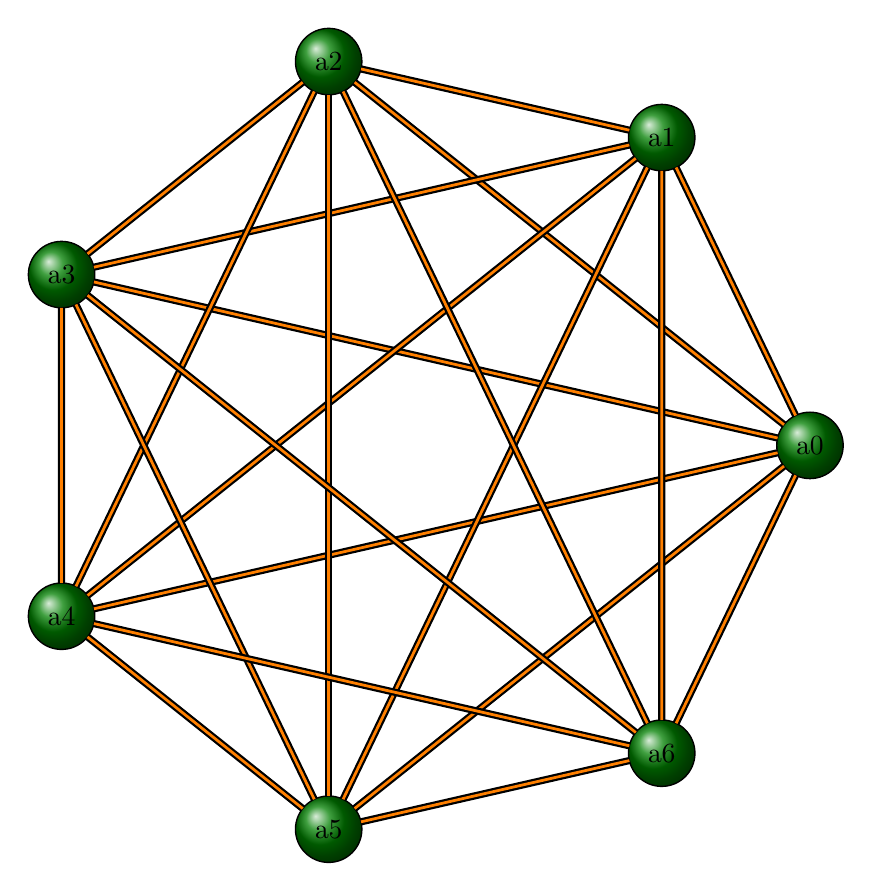
\begin{tikzpicture}
  \renewcommand*{\VertexBallColor}{green!50!black}
  \GraphInit[vstyle=Shade]
  \grComplete[RA=5]{7}
\end{tikzpicture}
\end{tkzexample}
\end{center}


\vfill\newpage\null 

\subsubsection{Complete Graph order 4}
\begin{center}
\begin{tkzexample}[vbox]
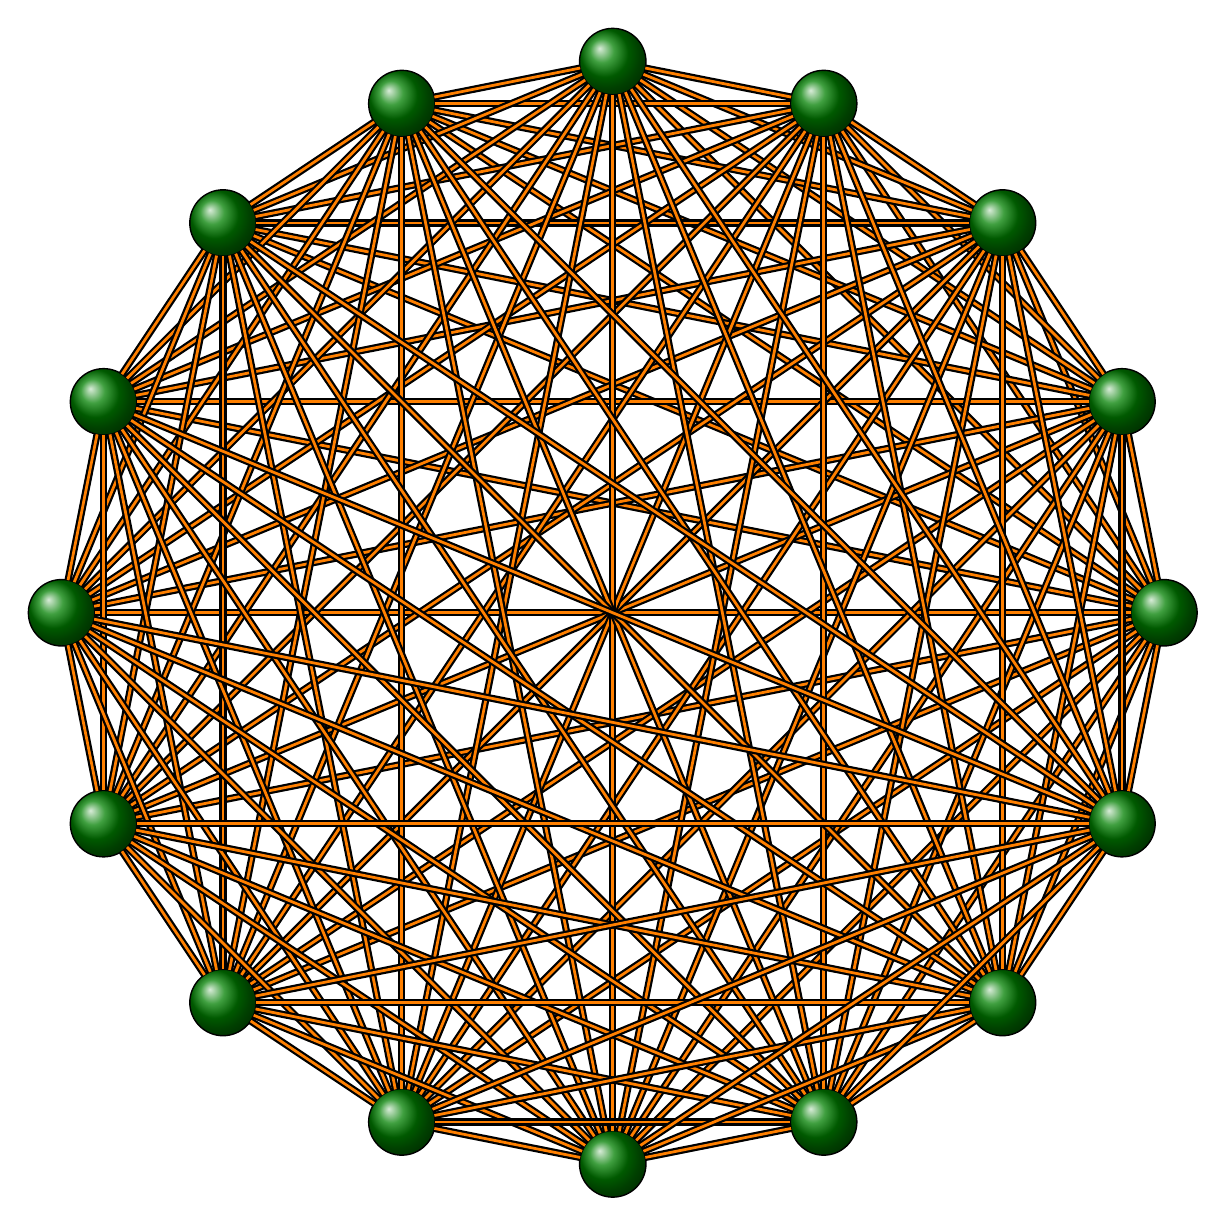
\begin{tikzpicture}
   \renewcommand*{\VertexBallColor}{green!50!black}
   \GraphInit[vstyle=Shade]
   \SetVertexNoLabel
   \grComplete[RA=7]{16}
\end{tikzpicture}
\end{tkzexample}
\end{center}

%<––––––––––––––––––––––––––––––––––––––––––––––––––––––––––––––––––––––––––>
%<––––––––––––––––––––––––––––––––––––––––––––––––––––––––––––––––––––––––––>
%<––––––––––––––––––––––––––––––––––––––––––––––––––––––––––––––––––––––––––>
\newpage 
\subsubsection{Circulant graph}
\begin{NewMacroBox}{grCirculant}{\oarg{local options}\var{order}}

\medskip
\emph{The circulant graph  is defined for any order $n$ at least 3, and every subset $L$ of integers which are less than or equal to $n/2$.  A circulant graph is a graph  in which the $i$th graph vertex is adjacent to the ($i+j$)th and ($i-j$)th graph vertices for each $j$ in a list $L$ . The circulant graphs with $L=\{1;\dots;[n/2]\}$  gives the complete graphs  and the circulant graph with $L=\{1\}$  gives the cyclic graphs. The Möbius ladders are examples of circulant graphs.\\
 In graph theory, a graph  whose adjacency matrix is circulant is called a circulant graph.\\
The circulant graph on  vertices on a list of nodes  is implemented as \tkzcname{grCirculant} in the \tkzname{tkz-berge.sty} package.}

\medskip
External links :

\href{http://mathworld.wolfram.com/CirculantGraph.html}%
           {\textcolor{blue}{MathWorld - CirculantGraph}} by %
      \href{http://en.wikipedia.org/wiki/Eric_W._Weisstein}%
           {\textcolor{blue}{E.Weisstein}}
\end{NewMacroBox}

\tikzset{VertexStyle/.style = {shape        = circle,
                               shading      = ball,
                               ball color   = green!40!black,%
                               minimum size = 16pt,%
                               draw}}
\SetUpEdge[style = {thick,%
                    double          = orange,%
                    double distance = 1pt}]

\SetVertexNoLabel
\tikzset{EdgeStyle/.style = {thick,
                             double= orange,
                             double distance = 1pt}} 

\subsubsection{ \opt{Graph  order 5 with L=\{1\}}}

This is a cycle graph.

\begin{center}
\begin{tkzexample}[vbox]
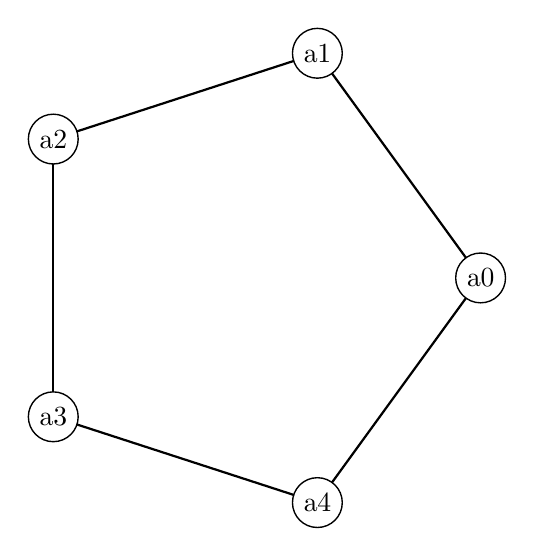
\begin{tikzpicture}
   \grCirculant[RA=3]{5}{1}%
\end{tikzpicture}
\end{tkzexample}
\end{center}

\subsubsection{\opt{Graph  order 5 with L=\{2\}}}

\begin{center}
\begin{tkzexample}[vbox]
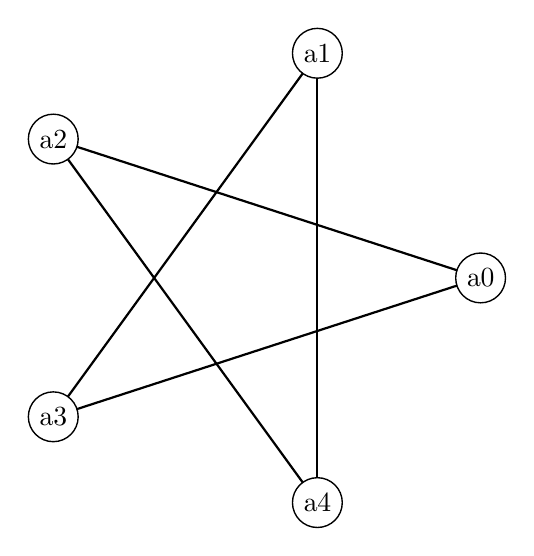
\begin{tikzpicture}
   \grCirculant[RA=3]{5}{2}%
\end{tikzpicture}
\end{tkzexample}
\end{center}


\subsubsection{\opt{Graph  order 5 with L=\{1,2\}}}

This graph is complete with an order $5$.

\begin{center}
\begin{tkzexample}[vbox]
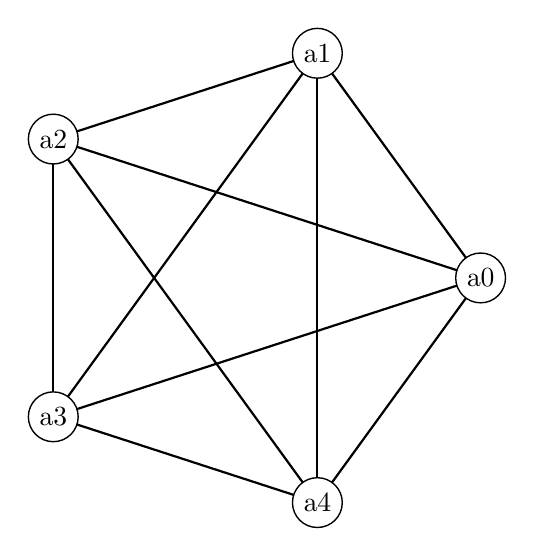
\begin{tikzpicture}
   \grCirculant[RA=3]{5}{1,2}%
\end{tikzpicture}
\end{tkzexample}
\end{center}


\subsubsection{\opt{Graph  order 10 with L=\{1,2,3,4,5\}}}

This graph is also complete

\begin{center}
\begin{tkzexample}[vbox]
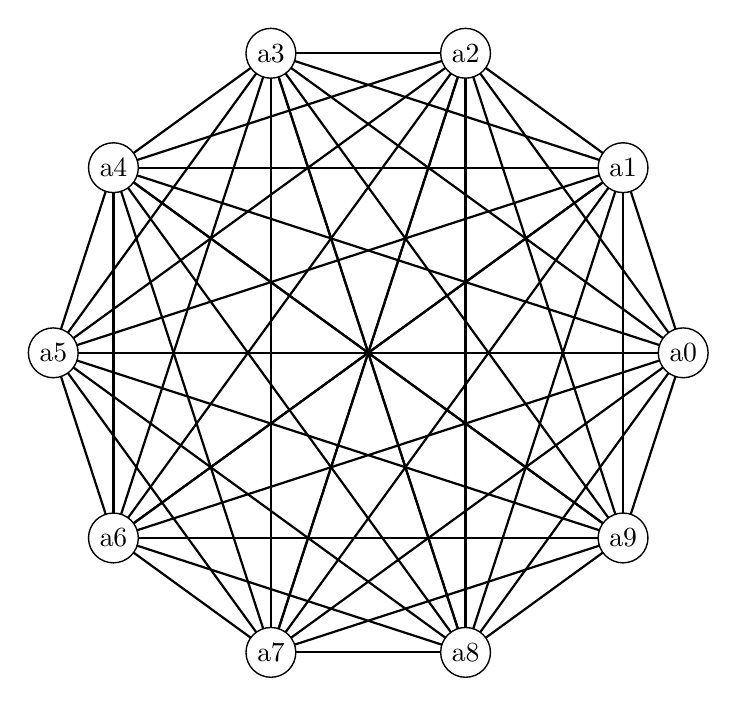
\begin{tikzpicture}
    \grCirculant[RA=4]{10}{1,2,3,4,5}%
\end{tikzpicture}
\end{tkzexample}
\end{center}

It's interesting to remark that the numbers 3 and 10 are primer, so if $L=\{3\} $ the graph is containing an Eulerian circuit.
 

\subsubsection{\opt{Graph  order 10 with L=\{3\}}}
\begin{center}
\begin{tkzexample}[vbox]
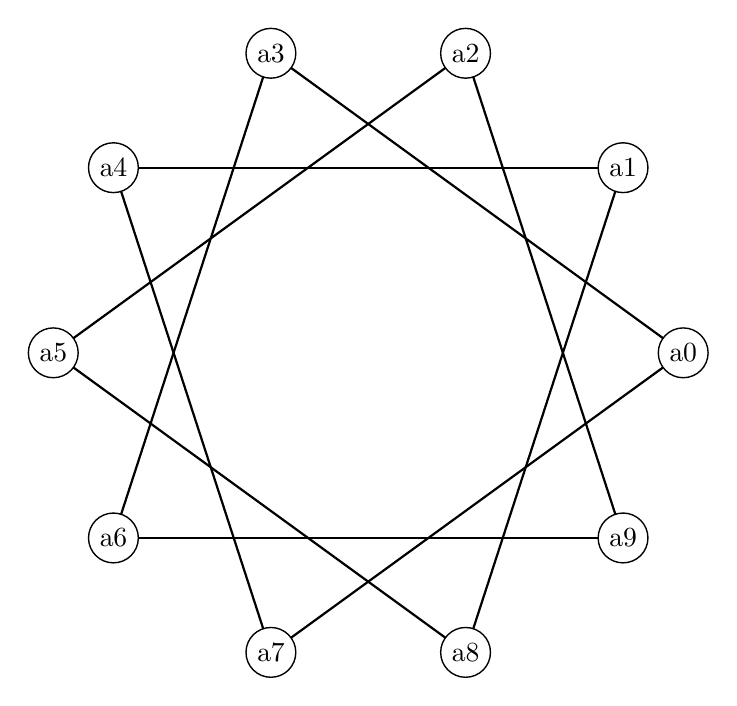
\begin{tikzpicture}
    \grCirculant[RA=4]{10}{3}%
\end{tikzpicture}
\end{tkzexample}
\end{center}

\vfill\newpage\null 
\tikzset{VertexStyle/.style = {shape           = circle,
                               shading         = ball,
                               ball color      = gray!30,%
                               minimum size    = 24pt,%
                               draw}}
\tikzset{EdgeStyle/.style = {thick,%
                               double          = orange,%
                               double distance = 1pt}} 
\SetVertexMath

\subsubsection{\opt{Graph  order 21 with L=\{1,3,10\}}}

\SetVertexNoLabel
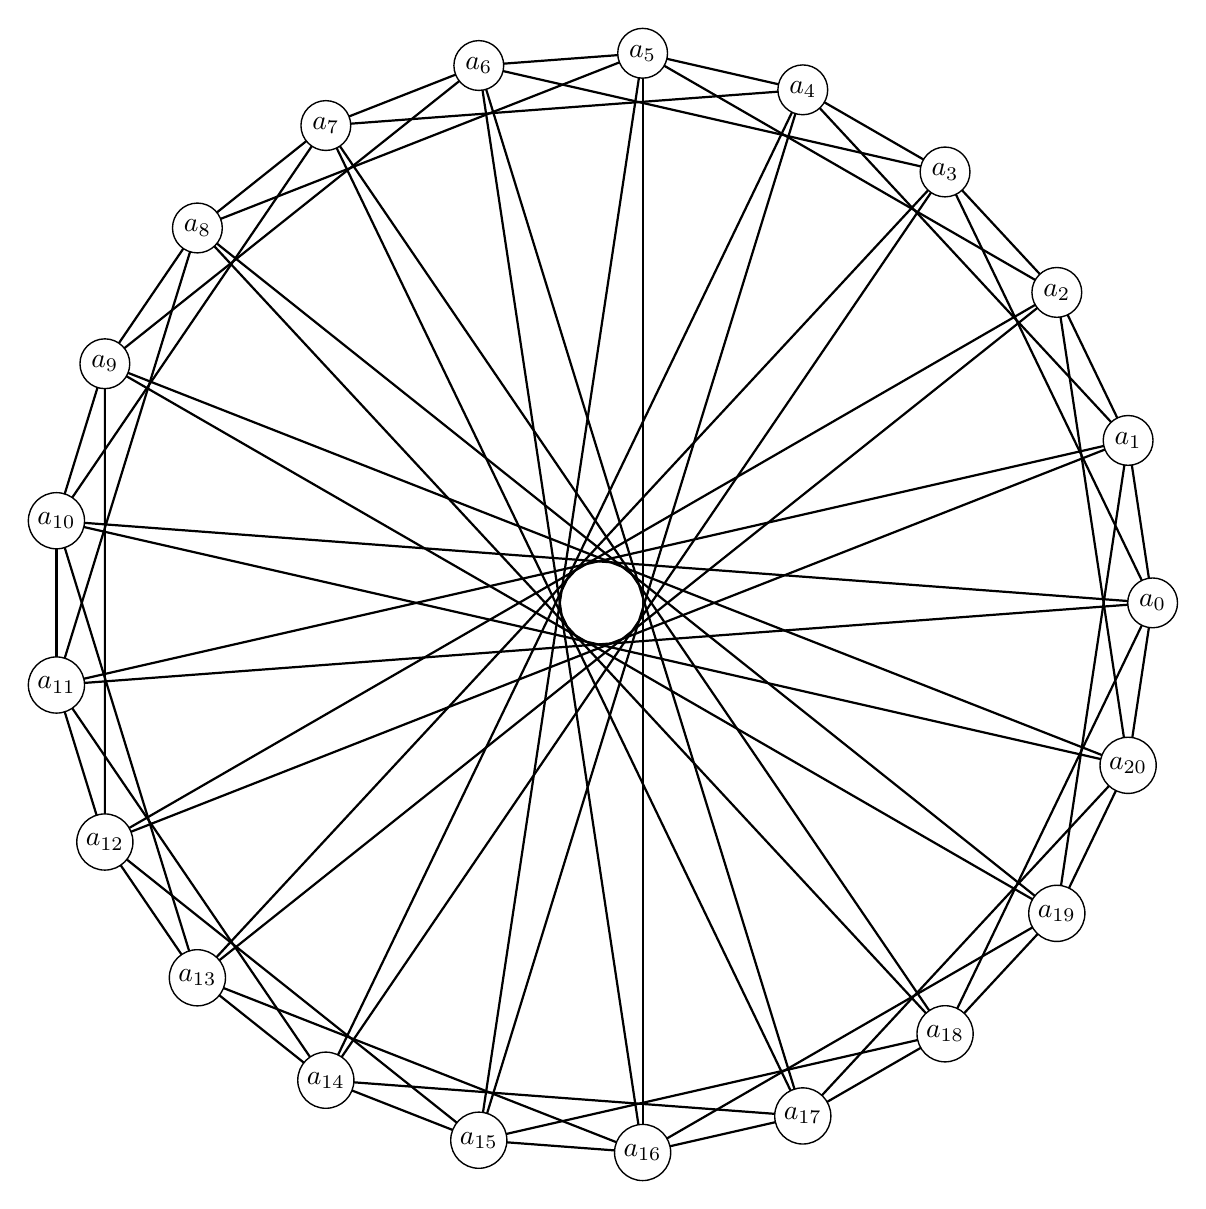
\begin{tikzpicture}
  \grCirculant[Math,RA=7]{21}{1,3,10}
\end{tikzpicture}
%<––––––––––––––––––––––––––––––––––––––––––––––––––––––––––––––––––––––––––>
%<–––––––––––––––––––––––––––   STAR    –––––––––––––––––––––––––––––––––––>
%<––––––––––––––––––––––––––––––––––––––––––––––––––––––––––––––––––––––––––>

\newpage 
\subsubsection{Star graph}  

\begin{NewMacroBox}{grStar}{\oarg{local options}\var{order}}

\medskip
\emph{A star graph $S_n$ is a n-graph   with one node having vertex degree $n-1$  and the other $n-1$   having vertex degree $1$. Star graphs can be generated using \tkzcname{grStar} in   the \tkzname{tkz-berge.sty} package.}

\medskip
External links :

\medskip
\begin{itemize}
\item \href{http://mathworld.wolfram.com/StarGraph.html}%
           {\textcolor{blue}{MathWorld - StarGraph}} by %
      \href{http://en.wikipedia.org/wiki/Eric_W._Weisstein}%
           {\textcolor{blue}{Weisstein}}
\end{itemize}
\end{NewMacroBox}

\tikzset{VertexStyle/.style = {shape        = circle,
                                 shading      = ball,
                                 ball color   = orange!40!,%
                                 minimum size = 26pt,%
                                 draw}}
\SetUpEdge[style={thick,%
           double          = orange,%
           double distance = 1pt}]
\SetVertexNoLabel
\tikzset{EdgeStyle/.style = {thick,
                             double= orange,
                             double distance = 1pt }}

\subsubsection{Star graph}
\begin{center}
  \begin{tkzexample}[vbox]
\begin{tikzpicture}[rotate=30,scale=.8]
  \grStar[RA=7]{8}%
\end{tikzpicture}
\end{tkzexample}
\end{center}

%<––––––––––––––––––––––––––––––––––––––––––––––––––––––––––––––––––––––––––>
%<––––––––––––––––––––––––––––––––––––––––––––––––––––––––––––––––––––––––––>
\newpage 
\subsubsection{Square graph} 

 \begin{NewMacroBox}{grSQCycle}{\oarg{local options}\var{Number}}

\medskip
\emph{A star graph $S_n$ is a n-graph   with one node having vertex degree $n-1$  and the other $n-1$   having vertex degree $1$. Star graphs can be generated using \tkzcname{grStar} in   the \tkzname{tkz-berge.sty} package.}

\medskip
External links :

\medskip
\begin{itemize}
\item \href{http://mathworld.wolfram.com/SquareGraph.html}%
           {\textcolor{blue}{MathWorld - SquareGraph}} by %
      \href{http://en.wikipedia.org/wiki/Eric_W._Weisstein}%
           {\textcolor{blue}{Weisstein}}
\end{itemize}
\end{NewMacroBox}

\subsubsection{Square Cycle graph}
\begin{center}
\begin{tkzexample}[vbox]
\begin{tikzpicture}[scale=.8]
  \grSQCycle[RA=7]{10}%
\end{tikzpicture}
\end{tkzexample}
\end{center}

%<––––––––––––––––––––––––––––––––––––––––––––––––––––––––––––––––––––––––––>
%<––––––––––––––––––––––––––––     WHEEL     –––––––––––––––––––––––––––––>
%<––––––––––––––––––––––––––––––––––––––––––––––––––––––––––––––––––––––––––>
\newpage 
\subsubsection{Wheel graph} 

\begin{NewMacroBox}{grWheel}{\oarg{local options}\var{Number}}

\medskip
\emph{A wheel graph   of order $n$  is a graph that contains a cycle of order $n-1$, and for which every  vertex in the cycle is connected to one other  vertex. The wheel  can be defined as the graph , where  is the singleton graph and  is the cycle graph.}

\medskip
External links :

\medskip
\begin{itemize}
\item \href{http://mathworld.wolfram.com/WheelGraph.html}%
           {\textcolor{blue}{MathWorld - WheelGraph}} by %
      \href{http://en.wikipedia.org/wiki/Eric_W._Weisstein}%
           {\textcolor{blue}{Weisstein}}
\end{itemize}
\end{NewMacroBox}

\tikzset{VertexStyle/.style = {shape        = circle,
                               shading      = ball,
                               ball color   = orange!40,%
                               minimum size = 24pt,%
                               draw}}
\SetUpEdge[style={thick,%
                  double          = orange,%
                  double distance = 1pt}]

\SetVertexNoLabel
\tikzset{EdgeStyle/.style = {thick,double= orange,double distance = 1pt}}
 
\vfill
\subsubsection{\tkzname{Wheel graph}}
\begin{center}
\begin{tkzexample}[vbox]
\begin{tikzpicture}[scale=.8]
      \grWheel[RA=7]{13}%
\end{tikzpicture}
\end{tkzexample}
\end{center}

%<––––––––––––––––––––––––––––––––––––––––––––––––––––––––––––––––––––––––––>
%<––––––––––––––––––––––––––––      LADDER        ––––––––––––––––––––––––––>
%<––––––––––––––––––––––––––––––––––––––––––––––––––––––––––––––––––––––––––>
\newpage 
\subsubsection{Ladder graph} 

\begin{NewMacroBox}{grLadder}{\oarg{local options}\var{Number}}

\medskip
\begin{tabular}{llc}
 \toprule   
options   & default  & definition                                           \\
\midrule
\TOline{RA     } { |4|    } {radius  circle n°1   }
\TOline{RS     } { |0|    } {distance between two lines } 
\TOline{prefix } { |a|    } {prefix for vertices        } 
\TOline{prefixx} { |b|    } {prefix for vertices        }       
\TOline{Math   } { |false|} {math mode                  }       
\bottomrule     
\end{tabular}

\medskip
\emph{The ladder graph $L_n$ or cyclic ladder graph is  equivalent to the grid graph  having two rails and $n$ rungs between them.}

\medskip
External links :

\medskip
\begin{itemize}
\item \href{http://mathworld.wolfram.com/LadderGraph.html}%
           {\textcolor{blue}{MathWorld - LadderGraph}} by %
      \href{http://en.wikipedia.org/wiki/Eric_W._Weisstein}%
           {\textcolor{blue}{Weisstein}}
\end{itemize}
\end{NewMacroBox}

\vfill
\subsubsection{\tkzname{Ladder graph}}
\begin{center}
\begin{tkzexample}[vbox]
\begin{tikzpicture}
      \grLadder[RA=2,RS=4]{6}%
\end{tikzpicture}
\end{tkzexample}
\end{center}

\vfill
%<––––––––––––––––––––––––––––––––––––––––––––––––––––––––––––––––––––––––––>
%<–––––––––––––––––––––––––––  Prism CYCLE LADDER     –––––––––––––––––––––––>
%<––––––––––––––––––––––––––––––––––––––––––––––––––––––––––––––––––––––––––>
\newpage 
\subsubsection{Prism graph} 

\begin{NewMacroBox}{grPrism}{\oarg{local options}\var{Number}}
  
\medskip
\begin{tabular}{llc}
 \toprule   
options   & default  & definition                                           \\
\midrule
\TOline{RA      } { |4|    }  {radius  circle n°1  }                             
\TOline{RB      } { |3|    }  {radius  circle n°2  }                             
\TOline{prefix  } { |a|    }  {prefix for vertices }                        
\TOline{prefixx } { |b|    }  {prefix for vertices }                 
\TOline{Math    } { |false|}  {math mode           }    
\bottomrule
\end{tabular}

\medskip
\emph{An $n$-prism graph has $2n$  nodes and $3n$ edges, and is equivalent to the generalized Petersen graph with arguments $n$ and $1$. For odd $n$, the $n$-prism is isomorphic to the circulant graph with an order $2n$ and with arguments $2$ and $n$.\\
The 3-prism graph   is the line graph of the complete bipartite graph with arguments $2$ and $3$ . The 4-prism graph  is isomorphic with the cubical graph.}


\medskip
External links :

\medskip
\begin{itemize}
\item \href{http://mathworld.wolfram.com/PrismGraph.html}%
           {\textcolor{blue}{MathWorld - Prism Graph}} by %
      \href{http://en.wikipedia.org/wiki/Eric_W._Weisstein}%
           {\textcolor{blue}{Weisstein}}
\end{itemize}
\end{NewMacroBox}

\subsubsection{\tkzname{Cycle Ladder graph}}
\begin{center}
\begin{tkzexample}[vbox]
\begin{tikzpicture}[rotate=15,scale=.7]
  \grPrism[RA=6,RB=3]{6}%
\end{tikzpicture}
\end{tkzexample}
\end{center}


\subsubsection{\tkzname{Cycle Ladder graph number 3}}
\begin{center}
\begin{tkzexample}[]
\begin{tikzpicture}[scale=.7]
  \grPrism[RA=6,RB=3]{3}%
\end{tikzpicture}
\end{tkzexample}
\end{center}


\subsubsection{\tkzname{Cycle Ladder graph number 4}}
\begin{center}
\begin{tkzexample}[]
\begin{tikzpicture}[scale=.7] 
  \grPrism[RA=6,RB=3]{4}%
\end{tikzpicture}
\end{tkzexample}
\end{center}


%<––––––––––––––––––––––––––––––––––––––––––––––––––––––––––––––––––––––––––>
%<–––––––––––––––––––––––––––––   bipartite ––––––––––––––––––––––––––––––––>
%<––––––––––––––––––––––––––––––––––––––––––––––––––––––––––––––––––––––––––>
\newpage 
\subsubsection{Complete Bipartite graph} 

\begin{NewMacroBox}{grCompleteBipartite}{\oarg{local options}\var{Number 1}\var{Number 2}}

\medskip
\begin{tabular}{llc}
 \toprule   
options   & default  & definition                                           \\
\midrule
\TOline{RA     }{|4|     } {radius  circle n°1}    
\TOline{RB     }{|3|     } {radius  circle n°2 }  
\TOline{RS     }{|1|     } {distance between two lines }
\TOline{form   }{|1|     } {integer to obtain a new embedding of a graph}
\TOline{prefix }{|a|     } {prefix for vertices  }
\TOline{prefixx}{|b|     } {prefix for vertices }
\TOline{Math   }{|false| } {math mode }
\bottomrule
\end{tabular}

\medskip
\emph{A complete bipartite graph is a bipartite graph (i.e., a set of graph vertices decomposed into two disjoint sets such that no two graph vertices within the same set are adjacent) such that every pair of graph vertices in the two sets are adjacent.}

\medskip
External links :

\medskip
\begin{itemize}
\item \href{http://mathworld.wolfram.com/CompleteBipartiteGraph.html}%
           {\textcolor{blue}{MathWorld - CompleteBipartite Graph}} by %
      \href{http://en.wikipedia.org/wiki/Eric_W._Weisstein}%
           {\textcolor{blue}{Weisstein}}
\end{itemize}
\end{NewMacroBox}   



\subsubsection{\tkzname{Bipartite graph 1,5}}\label{cl17}
\begin{center}
\begin{tkzexample}[vbox]
\begin{tikzpicture}
   \grCompleteBipartite[RA=4,RB=2.5,RS=4]{1}{5}
\end{tikzpicture}
\end{tkzexample}
\end{center}

\subsubsection{\tkzname{Bipartite graph 3,5}}\label{bi1}
\begin{center}
\begin{tkzexample}[vbox]
\begin{tikzpicture}
   \grCompleteBipartite[RA=4,RB=3,RS=6]{3}{5}
\end{tikzpicture}
\end{tkzexample}
\end{center}

%<––––––––––––––––––––––––––––––––––––––––––––––––––––––––––––––––––––––––––>
%<––––––––––––––––––––––––––––––––––––––––––––––––––––––––––––––––––––––––––>
%<––––––––––––––––––––––––––––––––––––––––––––––––––––––––––––––––––––––––––>
\newpage 
\subsubsection{Triangular Grid graph} 


\begin{NewMacroBox}{grTriangularGrid}{\oarg{local options}\var{Number}}

\medskip
\begin{tabular}{llc}
 \toprule   
options   & default  & definition                                           \\
\bottomrule
\TOline{RA    }{|4|    }{distance between two vertices   }
\TOline{form  }{|1|    }{integer to obtain a new embedding of a graph} 
\TOline{prefix}{|a|    }{prefix for vertices }
\TOline{Math  }{|false|}{math mode  }
\bottomrule
\end{tabular}

\emph{\tkzname{Number=$n$} is the number of vertices of the first row then the graph order is $\dfrac{n(n-1)}{2} $.
There are three embeddings. You can use the option \tkzname{form} with an integer between $1$ and $3$.}
\end{NewMacroBox} 

\medskip


\subsubsection{\opt{n=8 order=$28$} form 1}\label{cl18a}
\begin{center}
\begin{tkzexample}[vbox]
\begin{tikzpicture}
  \GraphInit[vstyle=Shade]
  \SetVertexLabel
  \grTriangularGrid[prefix=G,Math,RA=1.5]{8}%
\end{tikzpicture}
\end{tkzexample}
\end{center}

\subsubsection{\opt{n=6 order=$15$} form 2}
\begin{center}
\begin{tkzexample}[vbox]
\begin{tikzpicture}
  \GraphInit[vstyle=Shade]
  \SetVertexNoLabel
  \grTriangularGrid[RA=2,form=2]{6}%
\end{tikzpicture}
\end{tkzexample}
\end{center}


\subsubsection{\opt{n=6 order=$15$} form 3}
\begin{center}
\begin{tkzexample}[vbox]
\begin{tikzpicture}
  \GraphInit[vstyle=Shade]
  \SetVertexNoLabel
  \grTriangularGrid[RA=2,form=3]{6}%
\end{tikzpicture}
\end{tkzexample}
\end{center}
%<––––––––––––––––––––––––––––––––––––––––––––––––––––––––––––––––––––––––––>
\newpage 
\subsubsection{\tkzname{LCF Lederberg-Coxeter-Fruchte}}   

\begin{NewMacroBox}{grLCF}{\oarg{RA=\meta{Number}}  \var{List of numbers} \var{Number}}
\emph{LCF = Lederberg-Coxeter-Fruchte (see the link below for some examples).}

\medskip
External links :

\medskip
\begin{itemize}
\item \href{http://mathworld.wolfram.com/LCFNotation.html}%
           {\textcolor{blue}{MathWorld-LCF Notation}} by %
      \href{http://en.wikipedia.org/wiki/Eric_W._Weisstein}%
           {\textcolor{blue}{Weisstein}}
\end{itemize}
\end{NewMacroBox} 


\subsubsection{\tkzname{$\big[2,-2\big]^2$}}

\begin{center}
\begin{tkzexample}[vbox]
\begin{tikzpicture}%
       \grLCF[RA=5]{2,-2}{2}%
\end{tikzpicture}
\end{tkzexample}
\end{center}



\subsubsection{\tkzname{$\big[3,-3\big]^4$}}

\begin{center}
\begin{tkzexample}[vbox]
\begin{tikzpicture}%
       \grLCF[RA=5]{3,-3}{4}%
\end{tikzpicture}
\end{tkzexample}
\end{center}

\subsubsection{Ljubljana graph}
From Wikipedia \url{http://en.wikipedia.org/wiki/Ljubljana_graph}

\emph{The Ljubljana graph was first published in 1993 by Brouwer, Dejter and Thomassen.
In 1972, Bouwer was already talking of a 112-vertices edge- but not vertex-transitive cubic graph found by R. M. Foster, but unpublished. Conder, Malnič, Marušič, Pisanski and Potočnik rediscovered this 112-vertices graph in 2002 and named it the Ljubljana graph after the capital of Slovenia. They proved that it was the unique 112-vertices edge- but not vertex-transitive cubic graph and therefore that was the graph found by Foster.} 

It can be   represented in LCF notation as  :

\[ 
\begin{array}{l}
\Big[ 47, -23, -31, 39, 25, -21, -31, -41, 25, 15, 29, -41, -19, 15, -49, 33, 39, -35, -21, 17,\\ -33, 49, 41, 31, -15, -29, 41, 31, -15, -25, 21, 31, -51, -25, 23, 9, -17, 51, 35, -29, 21,\\ -51, -39, 33, -9, -51, 51, -47, -33, 19, 51, -21,29, 21, -31, -39\Big]^2 
\end{array} 
\]   

   
  \begin{center}
\begin{tikzpicture}
\GraphInit[vstyle=Art]
\SetGraphArtColor{black!50}{darkgray}
\tikzset{VertexStyle/.append style = {
                               minimum size         =  3pt}} 
       \grLCF[RA=7]{47, -23, -31, 39, 25, -21, -31, -41, 25, 15, 29, -41, -19, 15, -49, 33, 39, -35, -21, 17, -33, 49, 41, 31, -15, -29, 41, 31, -15, -25, 21, 31, -51, -25, 23, 9, -17, 51, 35, -29, 21, -51, -39, 33, -9, -51, 51, -47, -33, 19, 51, -21, 29, 21, -31, -39}{2}%  
\end{tikzpicture}
\end{center} 

\begin{tkzexample}[code only]
\GraphInit[vstyle=Art]
\SetGraphArtColor{black!50}{darkgray}
\tikzset{VertexStyle/.append style = {
                               minimum size         =  3pt}} 
\begin{tikzpicture}%
 \grLCF[RA=7]{47, -23, -31, 39, 25, -21, -31, -41, 25, 15, 29, -41, -19, 15,%
  -49, 33, 39, -35, -21, 17, -33, 49, 41, 31, -15, -29, 41, 31, -15, -25, 21,%
   31, -51, -25, 23, 9, -17, 51, 35, -29, 21, -51, -39, 33, -9, -51, 51, -47,%
    -33, 19, 51, -21, 29, 21, -31, -39}{2}%    
\end{tikzpicture}
\end{tkzexample} 
\vfill
\endinput

%!TEX root = /Users/ego/Boulot/TKZ/tkz-berge/doc-us/TKZdoc-berge-main.tex 
\section{Macros and Styles}

\subsection{How to change the background color and text color} 

You can use the following macro :

\begin{NewMacroBox}{tkzSetUpColors}{\oarg{local options}}

\begin{tabular}{llc}
  Options   & default  & definition                                  \\
\midrule
\TOline{background}  {white}      {couleur du fond  }             
\TOline{text} {black}   {couleur du texte }                                     
\end{tabular}
\end{NewMacroBox} 




\subsection{Modification of  labels \tkzcname{AssignVertexLabel}}

\begin{NewMacroBox}{AssignVertexLabel}{\oarg{local options}\var{prefix}\var{List of names}}
\begin{tabular}{lll}
  Arguments   &   & example                                  \\
\midrule
\TAline{prefix}        {}    {\tkzcname{AssignVertexLabel\{a\}\{Alter\}}}             
\TAline{List of names} {}    {\tkzcname{AssignVertexLabel\{a\}\{Paris,Lyon\}}}                        
\bottomrule
\end{tabular}

\medskip
\begin{tabular}{llc}
  Options   & default  & definition                                  \\
\midrule
\TOline{size}  {\tkzcname{normalsize}}      {taille de la fonte }             
\TOline{color} {black}   {couleur du texte }                       
\TOline{Math}   {false}  {math mode }                 
\end{tabular}
\end{NewMacroBox}

\medskip
\subsubsection{AssignStyle and \tkzcname{AssignVertexLabel}}
First step : We create an empty graph without labels.

Second step : We place labels with the macro \tkzcname{AssignVertexLabel} \begin{center}
\begin{tkzexample}[vbox]
\begin{tikzpicture}
  \SetVertexNoLabel
  \grCycle{6}
  \tikzset{AssignStyle/.append style = {below=12pt}}
  \AssignVertexLabel[color = blue,%
                     size  = \footnotesize]{a}{%
   Paris,Lyon,Marseille,Bordeaux,Reims,Saint-Etienne}
\end{tikzpicture}
\end{tkzexample}
\end{center}

\endinput     

\printindex  

\end{document}

\item \tkzcname{grHeawood}
\item \tkzcname{grGeneralizedPetersen}
\item \tkzcname{grPetersen}
\item \tkzcname{grTetrahedral}
\item \tkzcname{grOctahedral}
\item \tkzcname{grCubicalGraph}
\item \tkzcname{grIcosahedral}
\item \tkzcname{grDodecahedral}
\item \tkzcname{grMobiusKantor}
\item \tkzcname{grMobiusLadder}
\item \tkzcname{grCocktailParty}
\item \tkzcname{grCrown}
\item \tkzcname{grMcGee}
\item \tkzcname{grRobertson}
\item \tkzcname{grRobertsonWegner}
\item \tkzcname{grDoyle}
\item \tkzcname{grDesargues}
\item \tkzcname{grKonisberg}
\item \tkzcname{grWong}
\item \tkzcname{grTutteCoxeter}
\item \tkzcname{grFoster}
\item \tkzcname{grFolkman}
\item \tkzcname{grFranklin}
\item \tkzcname{grAndrasfai}
\item \tkzcname{grGrotzsch}
\item \tkzcname{grLevi}
\item \tkzcname{grPappus}
\item \tkzcname{grChvatal}
\item \tkzcname{grBalaban}

 